\section{Numerical solutions}\label{numerical}
In this section we numerically solve the linear stability problem
corresponding to Eq. \ref{lin_mass}---\ref{lin_energy}. 
We relax the thin-disk, low-frequency and nearly-Keplerian
approximations used in the analytical discussion above, and  
use the full expressions of $\rho$, $\Omega$ and
$\kappa$ given in \S\ref{eqm}. We also set $\hat{g}_c=1$ to
account for the background radial disk structure.  

We solve the linear problem by expanding the
perturbations in Chebyshev polynomials $T_l$ up to $l=512$
and discretizing the equations on a grid with
$z\in[-\zmax,\zmax]$. Our standard boundary conditions at the vertical
boundaries is a free surface, 
\begin{align}
  \Delta P \equiv \delta P + \bm{\xi}\cdot\nabla P= 0 \quad \text{at } z=\pm\zmax,
\end{align}
where $\bm{\xi}$ is the Lagrangian displacement, the meridional
components of which are given by $\xi_{x,z} = \ii\delta
v_{x,z}/\sigma$. 

The above discretization procedure
converts the linear system of differential equations to a set of 
algebraic equations, for which we use matrix routines in the LAPACK
package to solve. 

Unless otherwise stated, our fiducial disk model is: a nearly 
vertically isothermal disk with $\Gamma=1.011$, stable
stratification $\gamma=1.4$, $(p,q,\epsilon)=(-1.5,-1,0.05)$, and 
vertical domain size $\zmax=5H$. In Fig. \ref{omega_z} we plot the
corresponding equilibrium rotation profile, which shows that $\Omega$
decreases slightly away from the mid-plane.  

\begin{figure}
  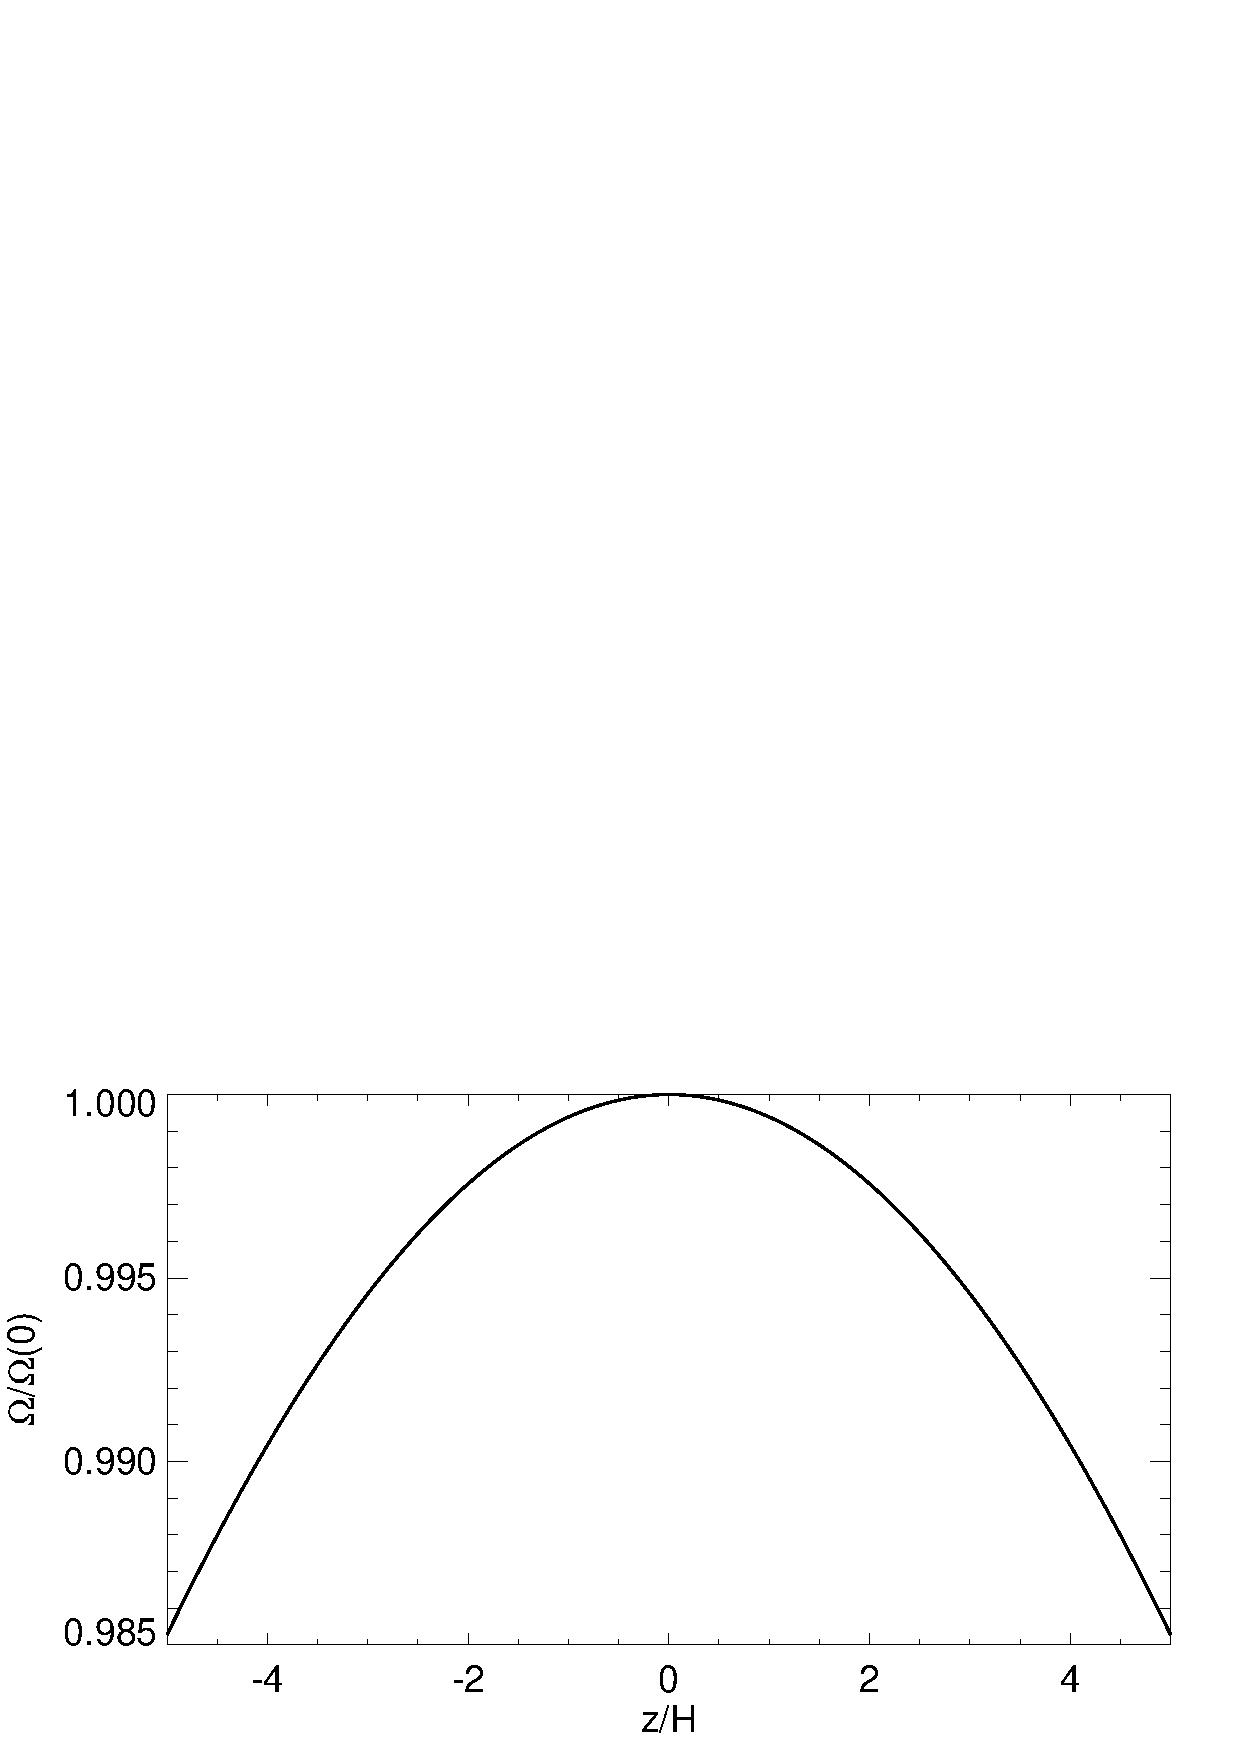
\includegraphics[width=\linewidth,clip=true,trim=0cm 0cm 0cm
  0cm]{figures/omega2} 
  \caption{Equilibrium rotation profile $\Omega(z)$,
    normalized by its mid-plane value, for a disk with $\Gamma=1.011$
    and $(p,q,\epsilon)=(-1.5,-1,0.05)$. 
    \label{omega_z} 
  }
\end{figure}

\subsection{VSI with rapid thermal relaxation}\label{vertiso_pertiso} 
We first calculate the VSI in a disk with rapid thermal relaxation by
setting $\beta=10^{-3}$. (Smaller values yield the same results.) This
is similar to strictly isothermal perturbations in a vertically
isothermal disk considered in \cite{nelson13} and \cite{mcnally14}. % We
% compare results with our analytical discussion of isothermal 
% perturbations in Appendix \ref{iso_discuss}. 

Fig. \ref{iso_eigen_kx} compares the numerically obtained eigenvalues 
for the fundamental mode and that calculated analytically from our
analysis of isothermal perturbations in Appendix \ref{iso_discuss}
(Eq. \ref{simple_growth} with $L=1$). We find good agreement in the
wave frequency $\omega$ at all $\khat$ and in growth rates $\nu$ for
$\khat\gtrsim 10$. Growth rates are $O(\epsilon\Omega_k)$, 
consistent with our discussion in Appendix \ref{max_growth1}, but
are over-estimated by our analysis. The match in $\nu$ worsens for
decreasing $\khat$ due to the neglect of global radial structure in
the  analysis. Nevertheless, given the number of approximations made
to calculate growth rates analytically, this agreement is
satisfactory, especially at large $\khat$.   

\begin{figure}
  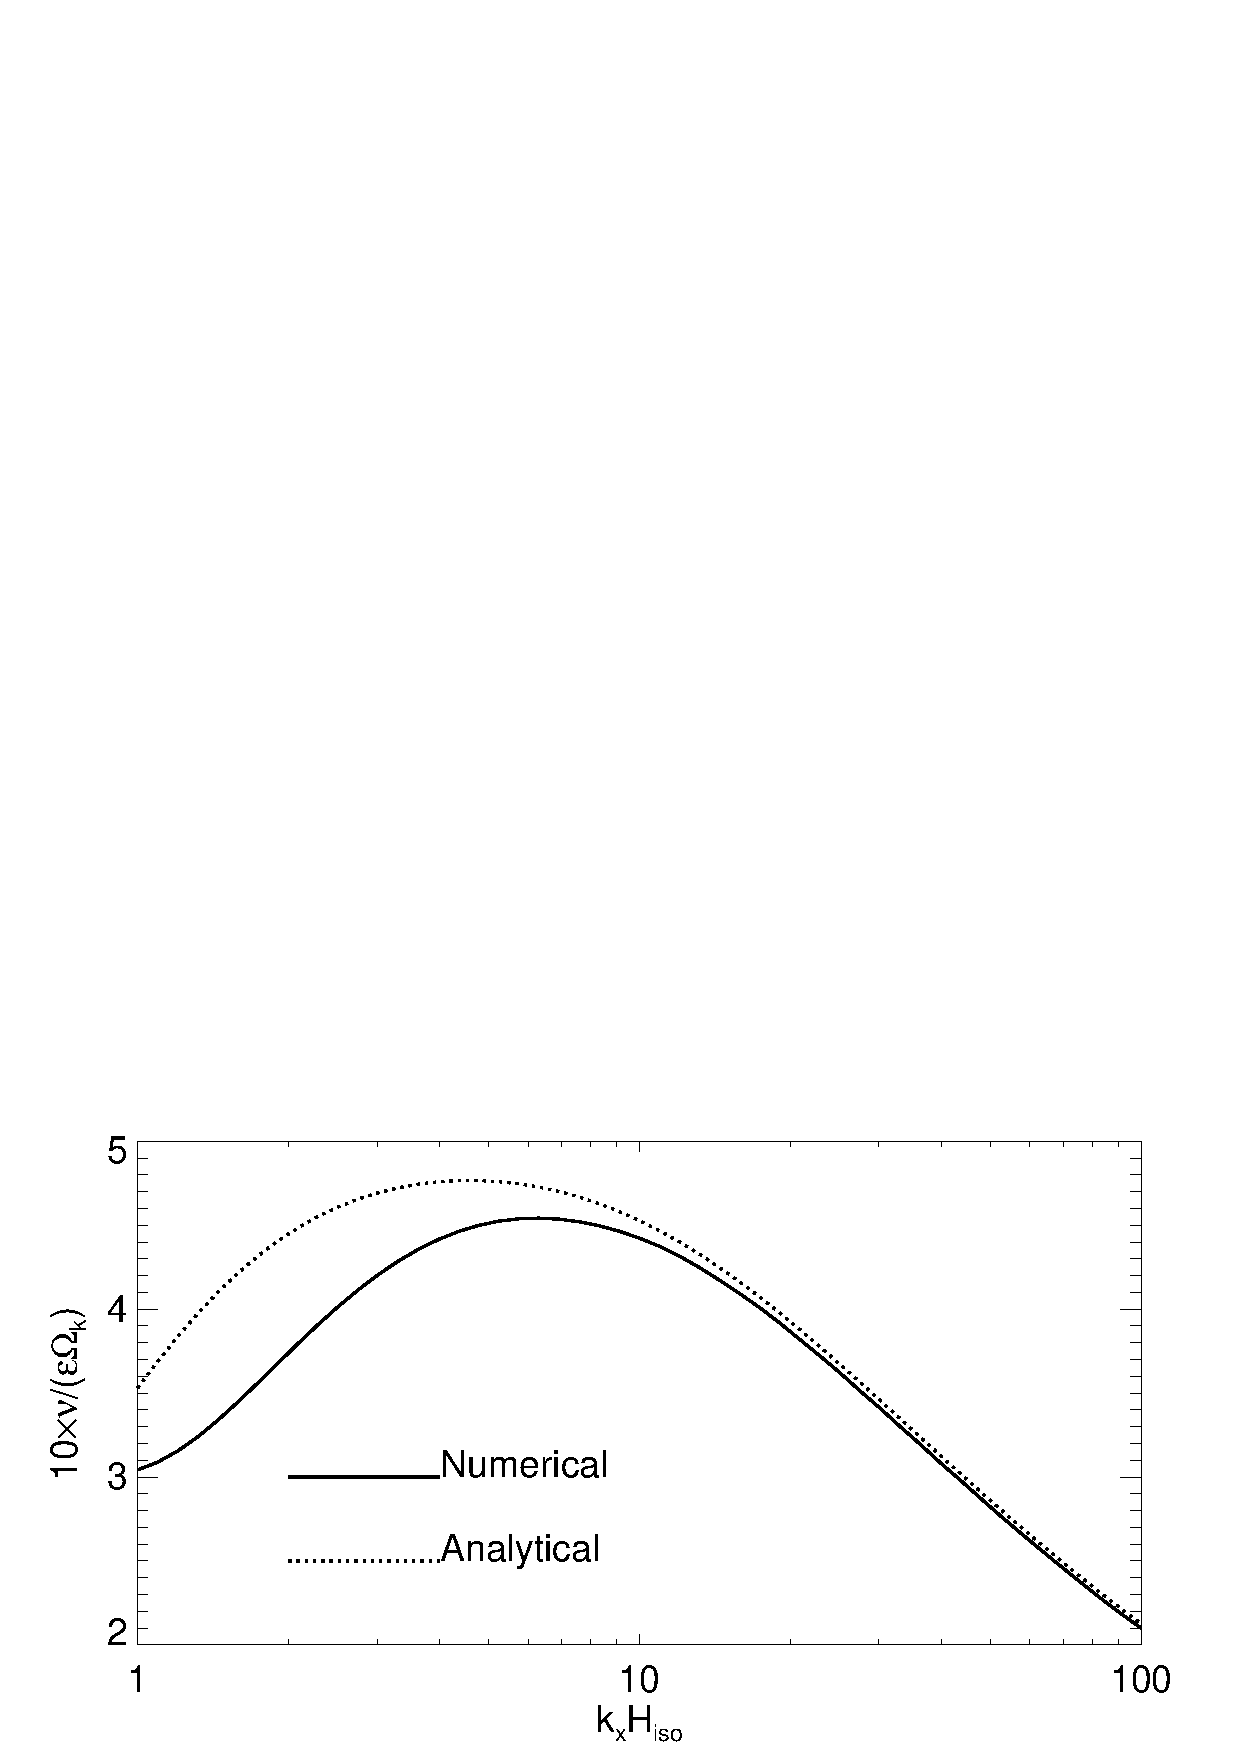
\includegraphics[width=\linewidth,clip=true,trim=0cm 1.75cm 0cm
  0cm]{figures/compare_eigen_imag_iso} 
  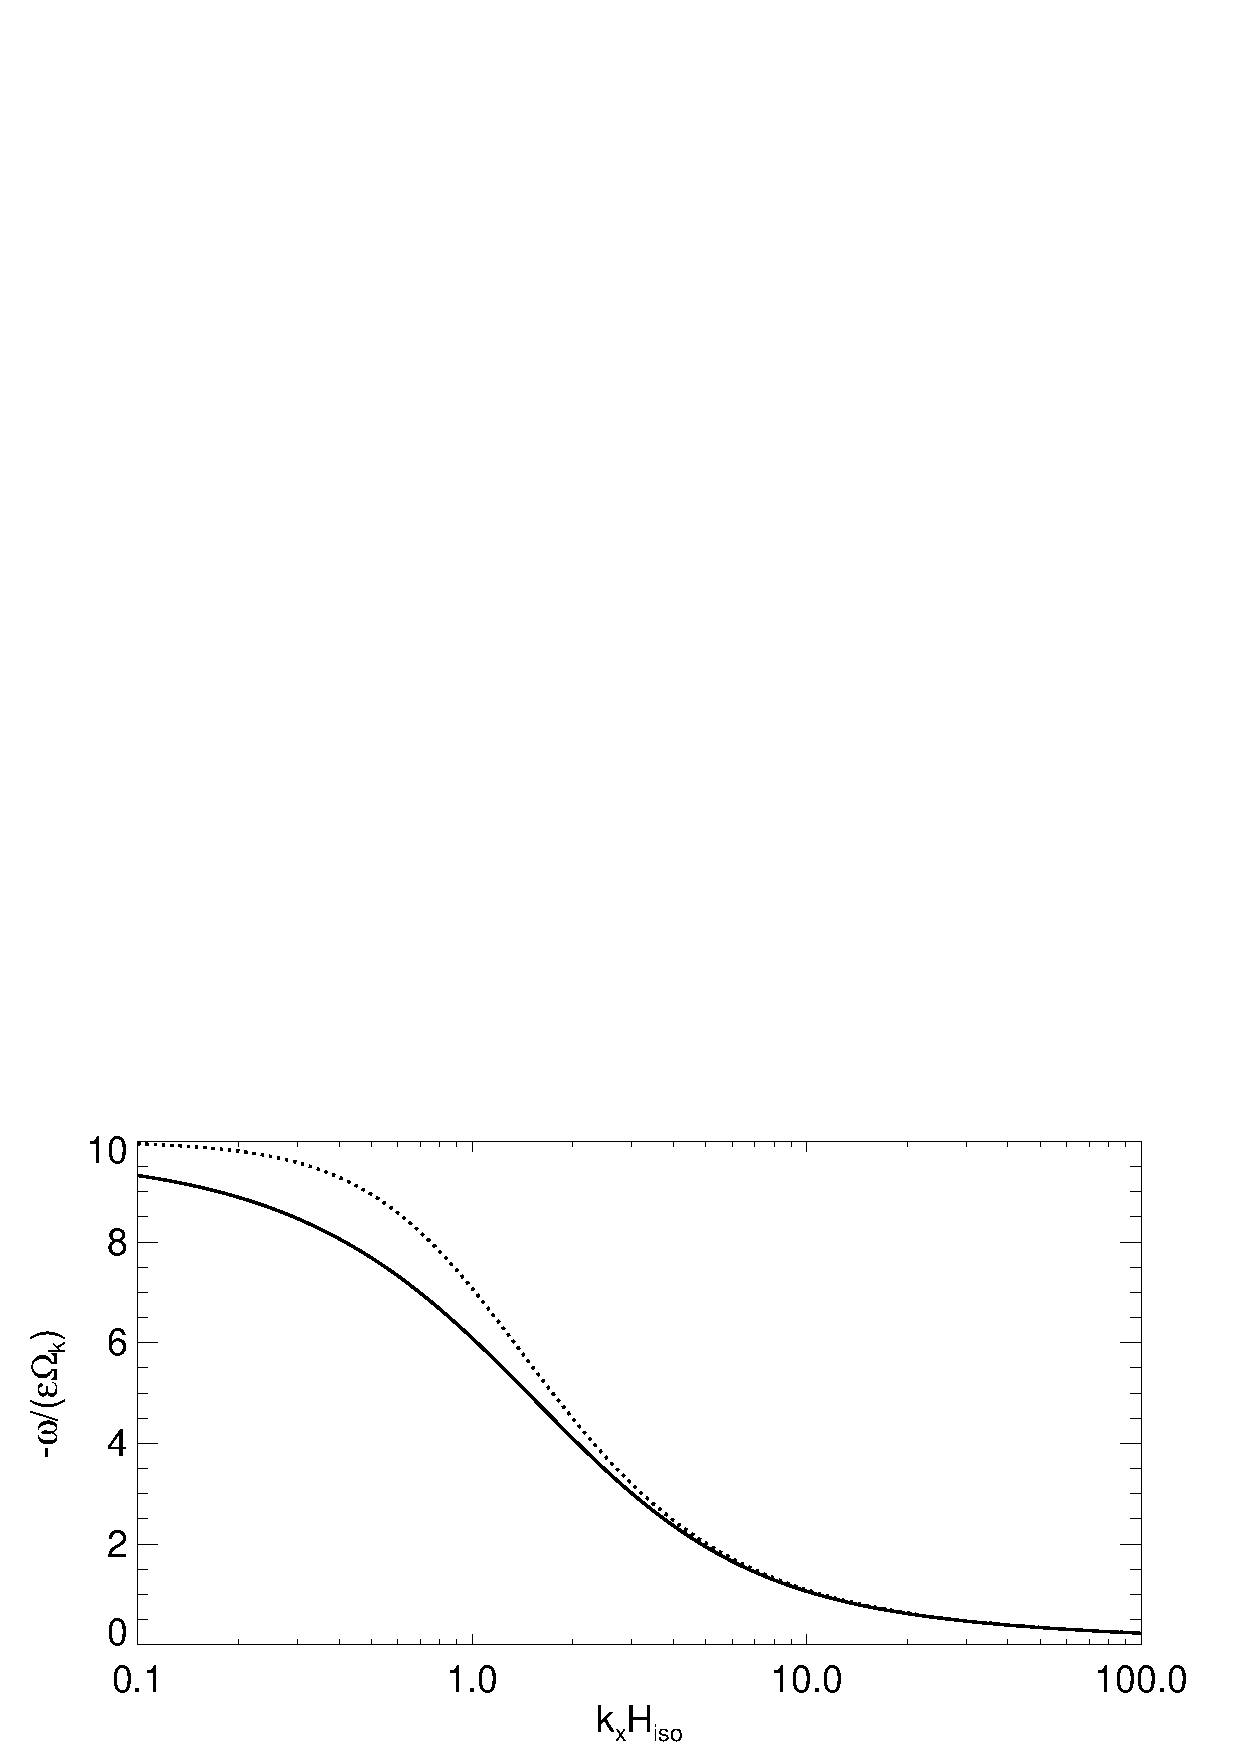
\includegraphics[width=\linewidth,clip=true,trim=0cm 0cm 0cm
  1cm]{figures/compare_eigen_real_iso}
  \caption{Growth rate (top) and real frequency (bottom) of the
    fundamental VSI mode in a disk with $(\gamma,
    \Gamma)=(1.4,1.011)$, $(p,q,\epsilon)=(-1.5,-1,0.1)$ and
    $\beta=10^{-3}$. The solid (dotted) line is obtained numerically
    (analytically).  
    \label{iso_eigen_kx} 
  }
\end{figure}

With rapid thermal relaxation, growth rates are expected to diminish for both $\khat\to 0$
and $\khat\to \infty$. This is because for $\khat\ll 1$ the radial
wavelenth is large, but such disturbances are 
stabilized by by epicyclic motions ($|\omega|\sim
\kappa$). Disturbances with $\khat\gg 1$ are radially localized, but  
there is no energy change when fluid elements are perturbed at fixed
cylindrical radius whilst conserving its angular momentum (since we
consider axisymmetric perturbations).  
 
Fig. \ref{lowfreq_eigenfunc} plots the eigenfunctions $W$ and $\delta 
v_z$ for the fundamental mode with $\khat=10$ (i.e. the mode with
maximum growth rate in Fig. \ref{iso_eigen_kx}). We find $W\propto z$
throughout most of the disk, corresponding to a constant vertical
velocity perturbation, as expected for the fundamental mode according
to explicit solutions developed in Appendix \ref{iso_explicit}. We
show a meridional visualization of this mode in
Fig. \ref{lowfreq_eigenfunc_2d}. Radial velocities are typically much
smaller than vertical velocities. Although there is a constant vertical
velocity throughout the fluid column, most of the momentum is
contained within $\sim 2H$ of the midplane due to the density
stratification. 

\begin{figure}
  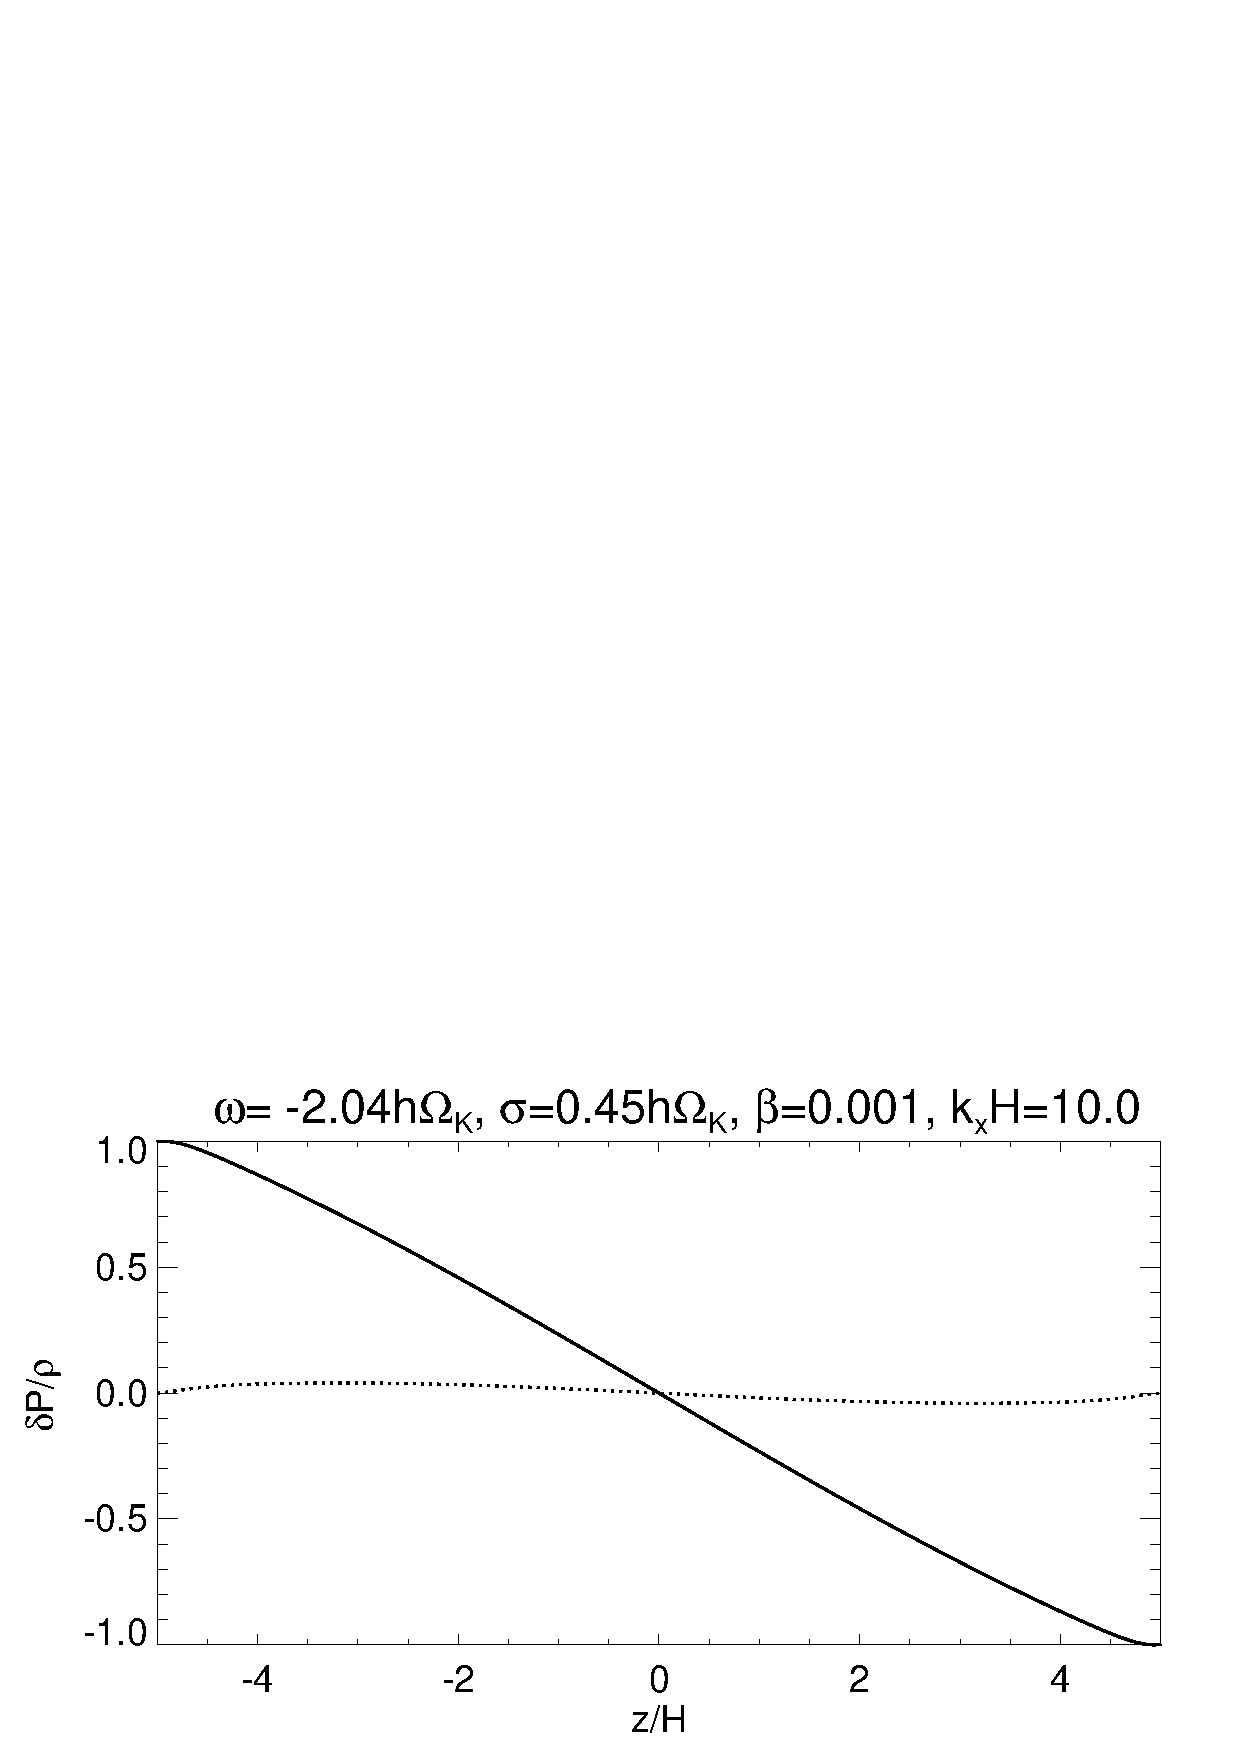
\includegraphics[width=\linewidth,clip=true,trim=0cm 1.75cm 0cm
  0cm]{figures/eigenvectorW_iso} 
  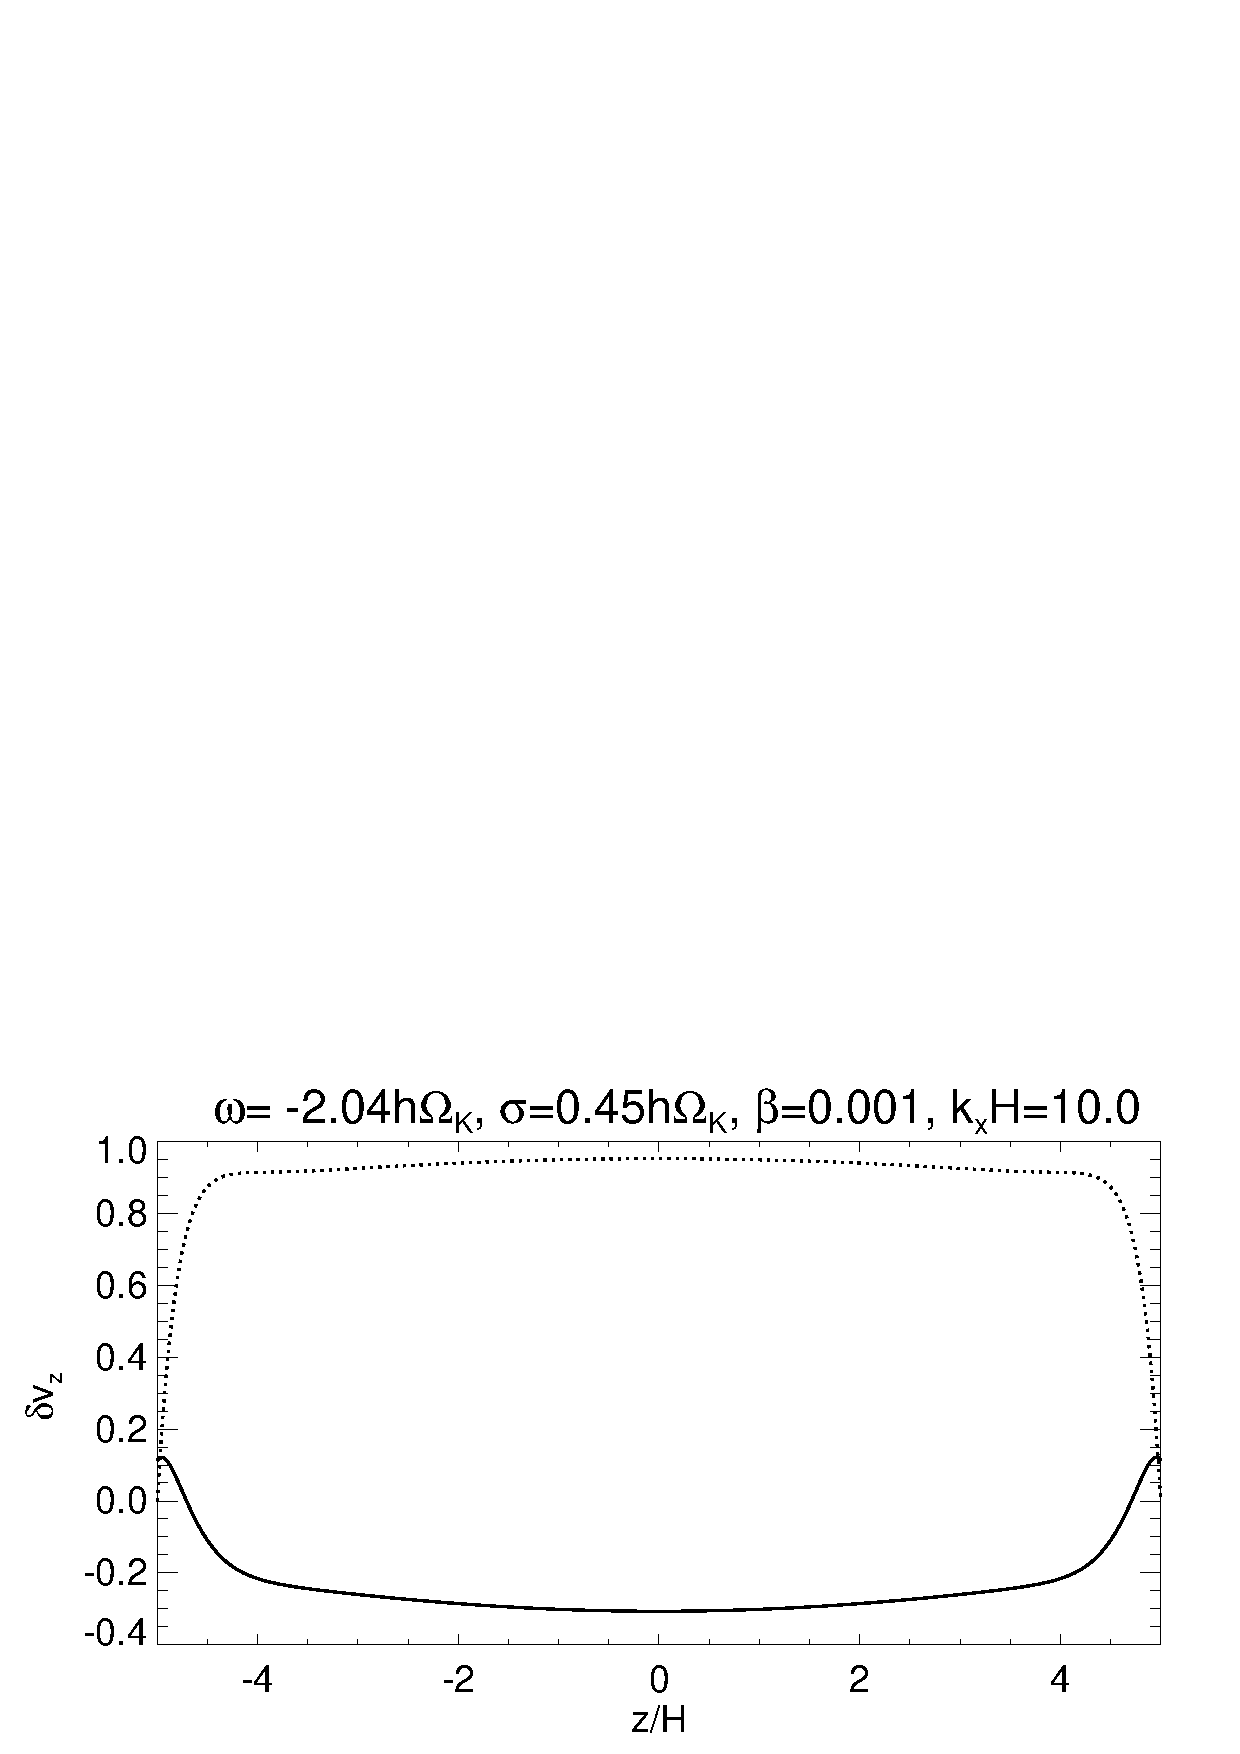
\includegraphics[width=\linewidth,clip=true,trim=0cm 0cm 0cm
  1cm]{figures/eigenvectorvz_iso}
  \caption{Pressure perturbation $W$ (top) and vertical velocity
    perturbation $\delta v_z$ of the fundamental VSI for a
    perturbation  wavenumber $\khat=10$  The real 
    (imaginary) parts of $W$ and $\delta v_z$ are plotted as solid
    (dotted) lines. 
    \label{lowfreq_eigenfunc}
  }
\end{figure}


\begin{figure}
  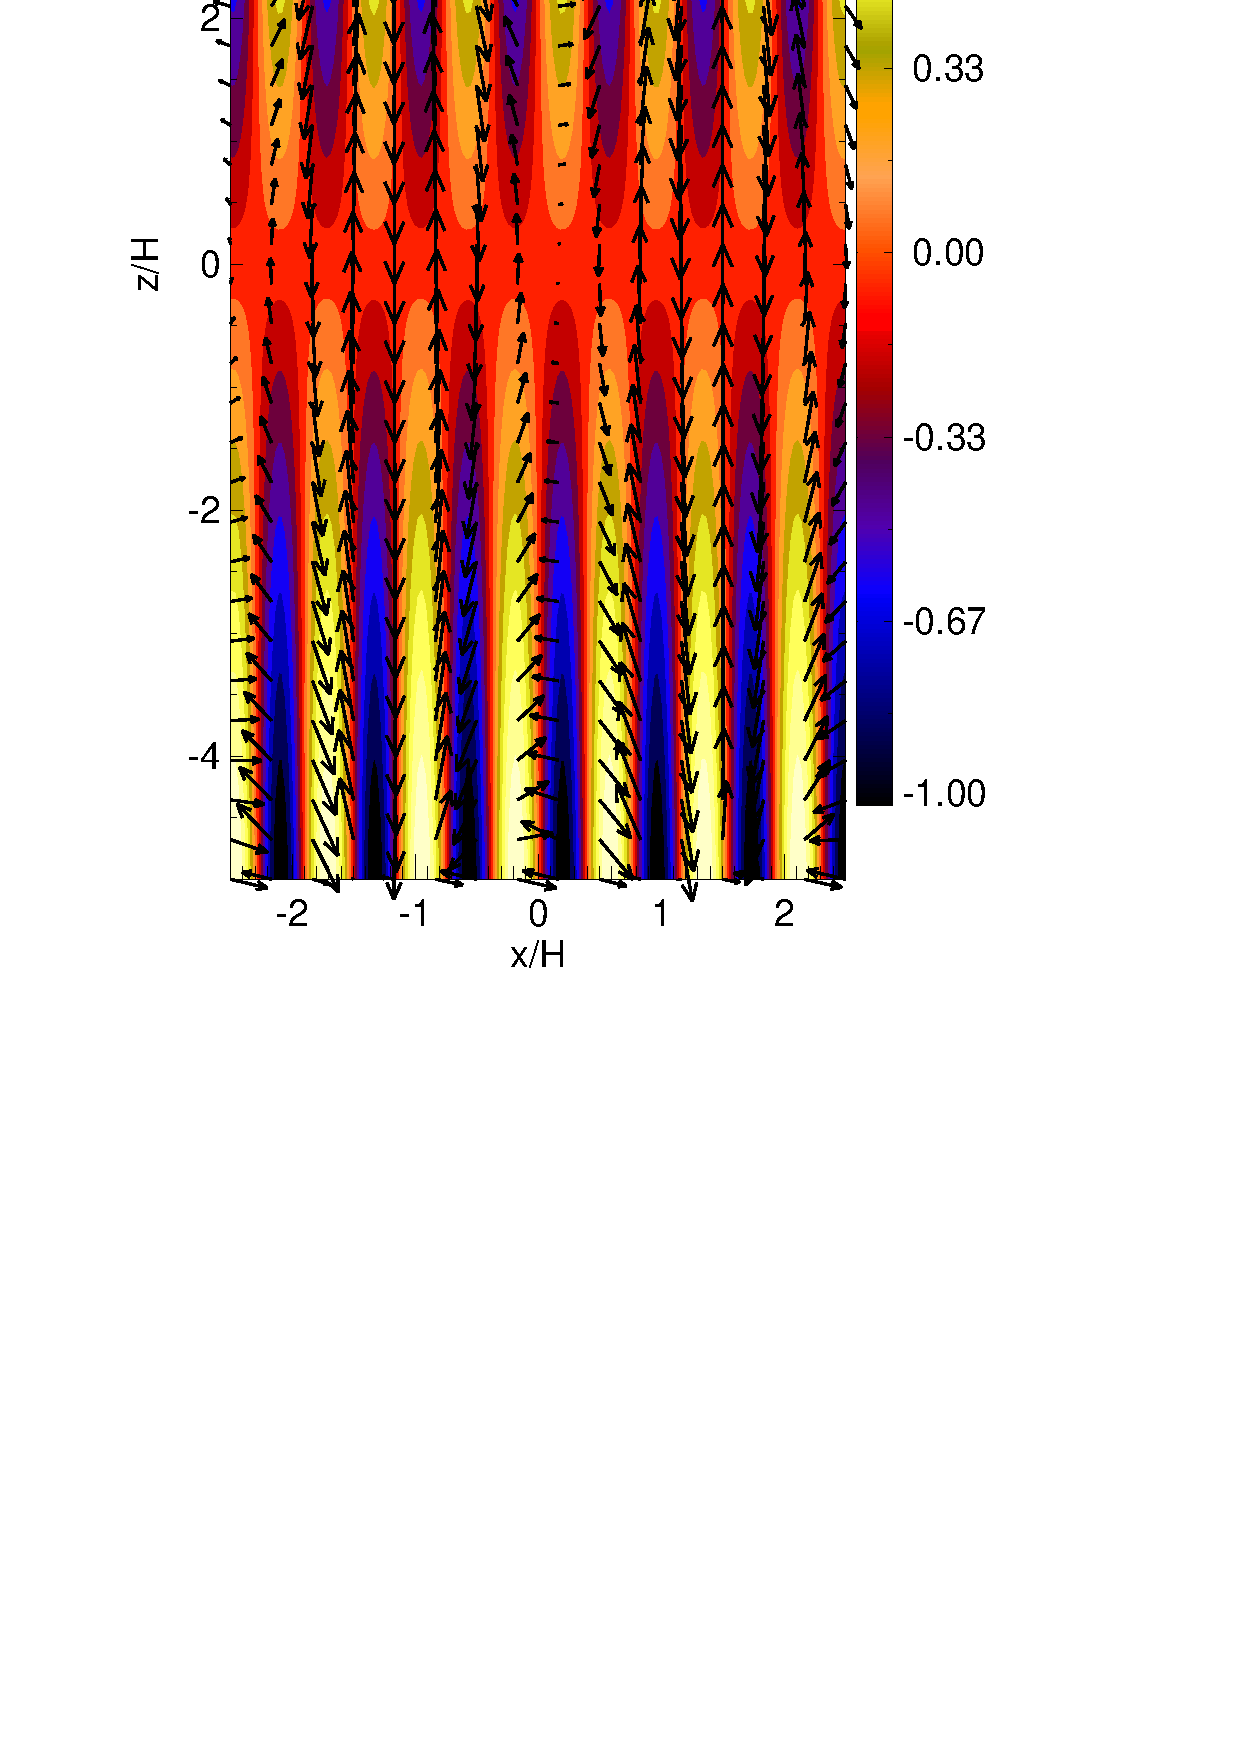
\includegraphics[scale=0.345,clip=true,trim=0cm 0cm 3.1cm
  0cm]{figures/result2d_vel}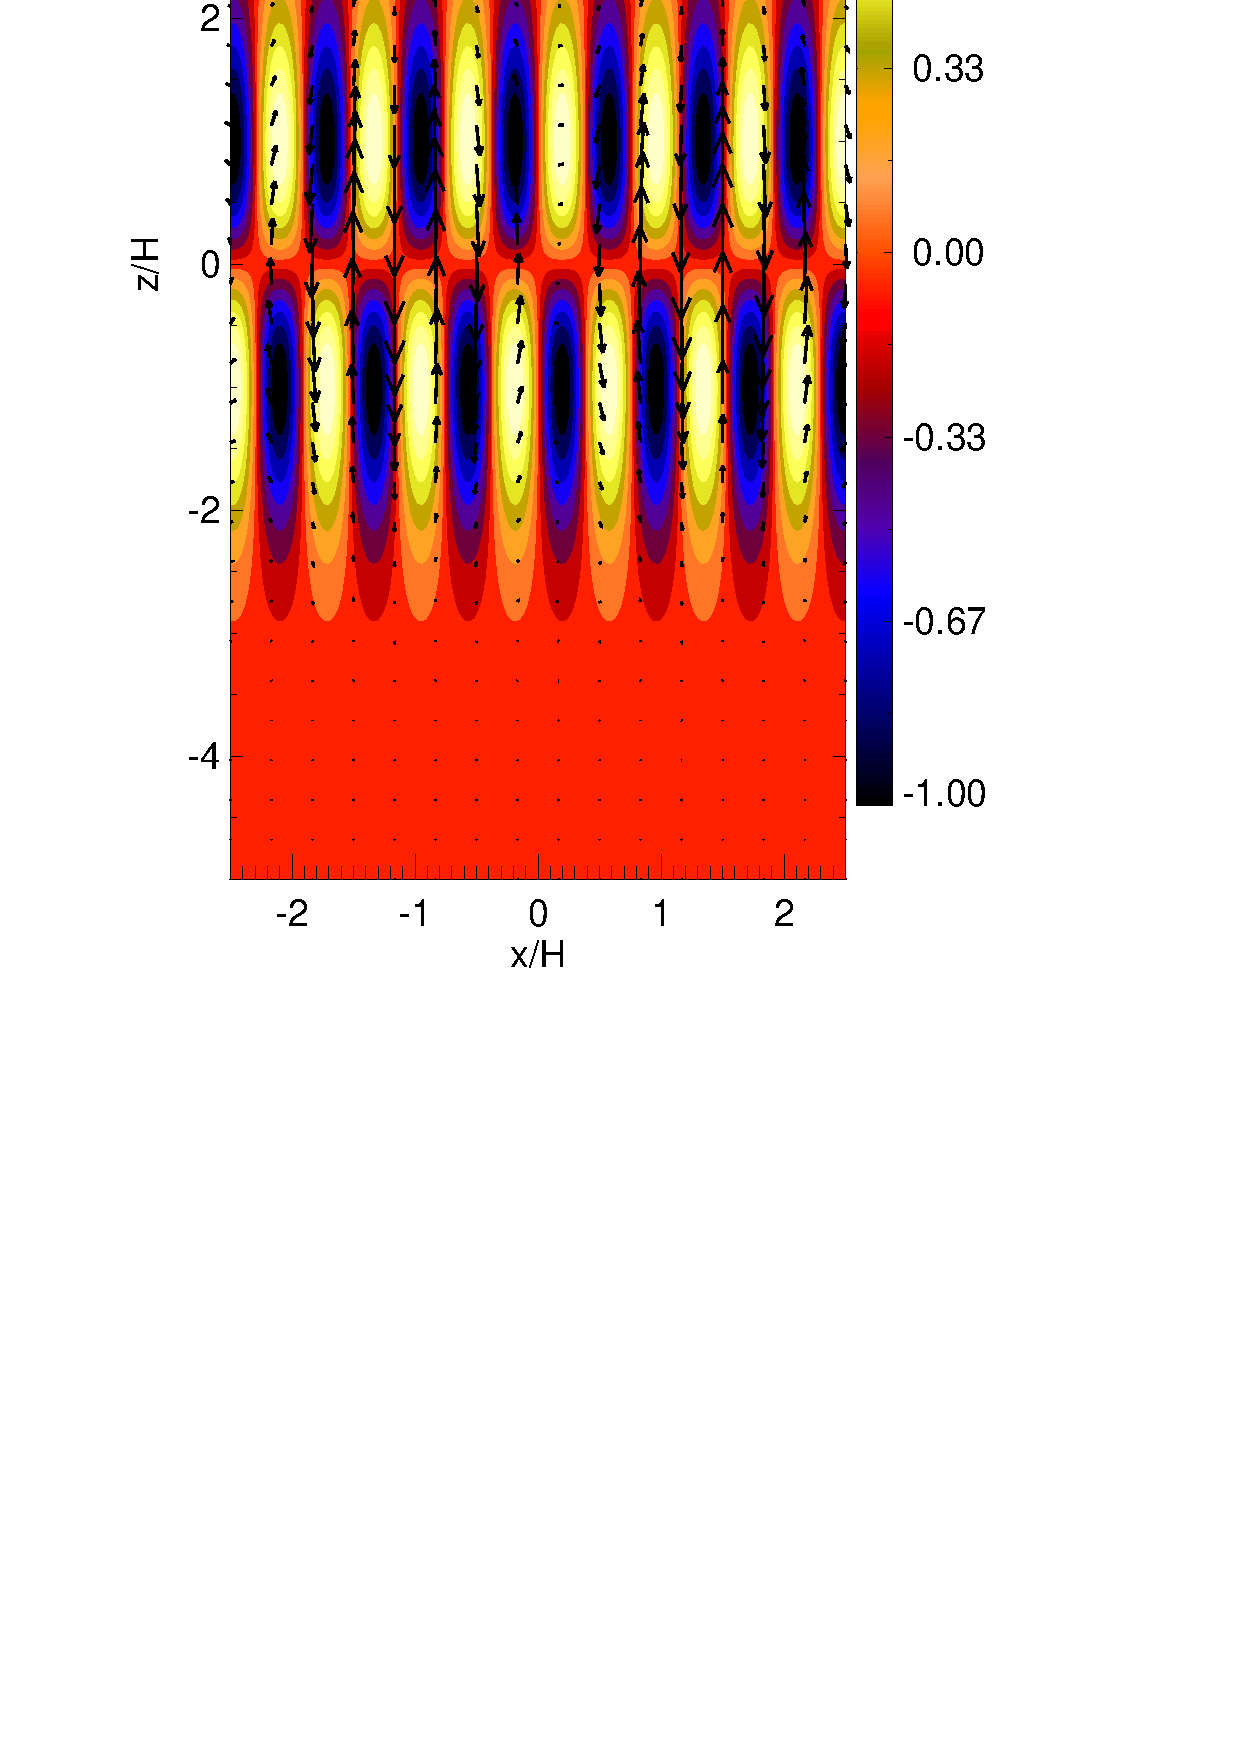
\includegraphics[scale=0.345,clip=true,trim=1.9cm 0cm 0cm
  0cm]{figures/result2d_mom} 
  \caption{Visualization of the fundamental VSI mode in
    Fig. \ref{lowfreq_eigenfunc}. The color scale corresponds to the
    real pressure perturbation $W$ scaled by its maximum value.
    Arrows in the left panel correspond to the meridional velocity
    field $(\delta v_x,\delta v_z)$, and arrows in the right panel
    correspond to to the meridional momentum $\rho(\delta v_x,\delta
    v_z)$. 
    \label{lowfreq_eigenfunc_2d}
  }
\end{figure}


\subsubsection{Case study: $\khat=10$}
In Fig. \ref{compare_modes_iso_kx10} we plot eigenvalues of unstable
modes found for our standard setup with $\khat=10$. This case is shown
by red crosses. We also plot several other calculations with different
vertical boundary conditions: free surface at $\zmax = 3H$ (black
dots), free surface at $\zmax=7H$ (green triangles) and a rigid
boundary at $\zmax=5H$ (blue cross).   

The fundamental mode, marked by `f', corresponds to the eigenvalue
with smallest magnitude $|\sigma|$. We see that the fundamental mode,
while not the most unstable in this case, is more robust against
vertical boundary conditions. Higher order modes with larger growth
rates (i.e. the branch where $\nu$ increases with $|\omega|$) require
larger vertical domains. 

\begin{figure}
  \includegraphics[width=\linewidth]{figures/compare_modes_iso_kx10.ps}
  \caption{Unstable modes for a disk with 
    $(\gamma,\Gamma)=(1.4,1.011)$, $(p,q,\epsilon)=(-1.5,-1,0.1)$ and
    $\beta=10^{-3}$. The perturbation wavenumber is $\khat=10$. 
    The standard setup with a free surface ($\Delta P=0$) and 
    vertical domain size $\zmax=5H$ is shown by the red cross. Other
    cases correspond to different boundary condtions applied at
    different heights. The fundamental mode is marked by `f'.   
    \label{compare_modes_iso_kx10} 
  }
\end{figure}

\subsubsection{Comment on `surface modes'} 
Our standard setup with $\khat=10$ in 
Fig. \ref{compare_modes_iso_kx10} (red crosses) differs to that from
\cite{nelson13} and \cite{mcnally14} in the lack of `surface modes' in
our case. These modes lie parallel to the vertical axis in mode
diagrams such as Fig. \ref{compare_modes_iso_kx10}. We find them for 
sufficiently large $\zmax$ and/or $\khat$. % For example, the two
% largest growth rates found for the case with $\zmax=7H$ in
% Fig. \ref{compare_modes_iso_kx10} are surface modes. 

To illustrate this, we plot the mode diagram for $\khat=30$ in  
Fig. \ref{compare_modes_iso_kx30} with different boundary 
conditions. Surface modes can be seen with
$\zmax\geq 5H$, examples of which are marked by `s'. These modes have
been discussed in the aforementioned studies. They typically have the
largest growth rates but require sufficiently large vertical domain
size and their eigenvalues vary with $\zmax$. 

Due to their dependence on boundary conditions, we
do not consider surface modes further in detail. In fact, we will see
in the next section that surface modes are more effectively stabilized
by finite thermal relaxation than the fundamental mode. %  Thus, surface
% modes may not be the most relevant in realistic disks.   

\begin{figure}
  \includegraphics[width=\linewidth]{figures/compare_modes_iso_kx30_tags.ps}
  \caption{Same as Fig. \ref{compare_modes_iso_kx10} but for $\khat=30$
    \label{compare_modes_iso_kx30}. Examples of surface modes are
    marked with `s'. These are found for sufficiently large vertical
    domain sizes. 
  }
\end{figure}


\subsection{Effect of thermal relaxation}\label{therm_relax_eff}
We now consider the effect of thermal relaxation by increasing
$\beta$. Note that for the standard disk model the critical thermal 
timescale $\beta_\mathrm{crit} = 0.125$.  

Fig. \ref{compare_modes_cool_kx10} show unstable modes with $\khat=10$
and $\beta\in[0.01,0.1]$. In addition to our standard setup with 
$\zmax=5H$, we also plot results for $\zmax=3H$ and $\zmax=7H$. In all
three cases the number of unstable modes decrease with increasing
$\beta$. The fundamental mode is not the most unstable for 
$\beta=0.01$ as there is a large number of higher order modes, but
these depend on boundary conditions.  

However, the fundamental mode is dominant for $\beta \geq 
0.03$. Higher order modes, with larger growth rates than the
fundamental mode, are more effectively stabilized with increasing 
$\beta$. For $\beta=0.1$, which is close to $\beta_\mathrm{crit}$, we
only find the fundamental mode. 

\begin{figure}
  \includegraphics[width=\linewidth,clip=true,trim=0cm 1.75cm 0cm
  0cm]{figures/compare_modes_cool_kx10_z3.ps} 
  \includegraphics[width=\linewidth,clip=true,trim=0cm 1.75cm 0cm
  0cm]{figures/compare_modes_cool_kx10_z5.ps}
  \includegraphics[width=\linewidth]{figures/compare_modes_cool_kx10_z7.ps}
  \caption{Unstable modes with $\khat=10$ and thermal
    relaxation timescales $\beta=0.01$ (black dots), $\beta=0.03$ (red
    crosses), $\beta=0.05$ (green triangles) and $\beta=0.1$ (blue
    crosses); for different vertical domain sizes $\zmax=3H$ (top),
    $\zmax=5H$ (middle, standard setup) and $\zmax=7H$ (bottom). The
    fundamental mode is marked with `f'. 
    \label{compare_modes_cool_kx10} 
  }
\end{figure}

Fig. \ref{compare_modes_cool_kx30} show unstable modes with
$\khat=30$. In this case surface modes appear for sufficiently large   
$\zmax$. However, they are effectively stabilized with increasing 
$\beta$. For $\zmax=3H$, the fundamental mode becomes dominant for
$\beta\geq 0.03$, as before. For $\zmax=5H$ and $\zmax=7H$, we find
the appearence of modes slightly more unstable than the fundamental
mode even when $\beta=0.1$ (the leftmost eigenvalues in the lower two
panels). However, these modes are clearly associated with the vertical
domain size as they are absent for $\zmax=3H$. % Thus, for $\zmax=5H$ and 
% $\zmax=7H$  the fundamental mode is likely dominant for 
% $\beta\geq0.05$  

\begin{figure}
  \includegraphics[width=\linewidth,clip=true,trim=0cm 1.75cm 0cm
  0cm]{figures/compare_modes_cool_kx30_z3.ps} 
  \includegraphics[width=\linewidth,clip=true,trim=0cm 1.75cm 0cm
  0cm]{figures/compare_modes_cool_kx30_z5.ps}
  \includegraphics[width=\linewidth]{figures/compare_modes_cool_kx30_z7.ps}
  \caption{Same as Fig. \ref{compare_modes_cool_kx10} but for
    $\khat=30$. Examples of surface modes are marked with `s', and 
    appear for sufficiently large $\zmax$.
    \label{compare_modes_cool_kx30} 
  }
\end{figure}

Fig. \ref{compare_modes_cool_kx10} and \ref{compare_modes_cool_kx30} 
show that the fundamental mode is not sensitive to boundary
conditions. Thus, tracking fundamental mode is a
more robust way of assessing stability as a function of $\beta$,
rather than searching for the most 
unstable mode, because the latter may be associated with boundary
conditions. In fact, the fundamental mode bcomes dominant 
(or close to it) with increasing $\beta$. 

Fig. \ref{lowfreq_eigenfunc_cool}---\ref{lowfreq_eigenfunc_2d_cool}
shows the fundamental mode with $\khat=10$ in a disk with 
$\beta=0.1$. These plots can be compared the case with rapid thermal
relaxation (Fig. \ref{lowfreq_eigenfunc}---\ref{lowfreq_eigenfunc_2d}). We see 
that increasing $\beta$ causes the region characterized by $W\sim z$ and  
$\delta v_z\sim$ constant closer to the mid-plane, with oscillatory
behavior emerging near vertical boundaries where buoyancy becomes
important. This leads to the `tilted' pressure perturbations seen in
Fig. \ref{lowfreq_eigenfunc_2d_cool}
(cf. Fig. \ref{lowfreq_eigenfunc_2d}). However, most of the meridional
momentum is still contained within $|z|\lesssim 2H$ as for 
the case with $\beta=10^{-3}$.  

\begin{figure}
  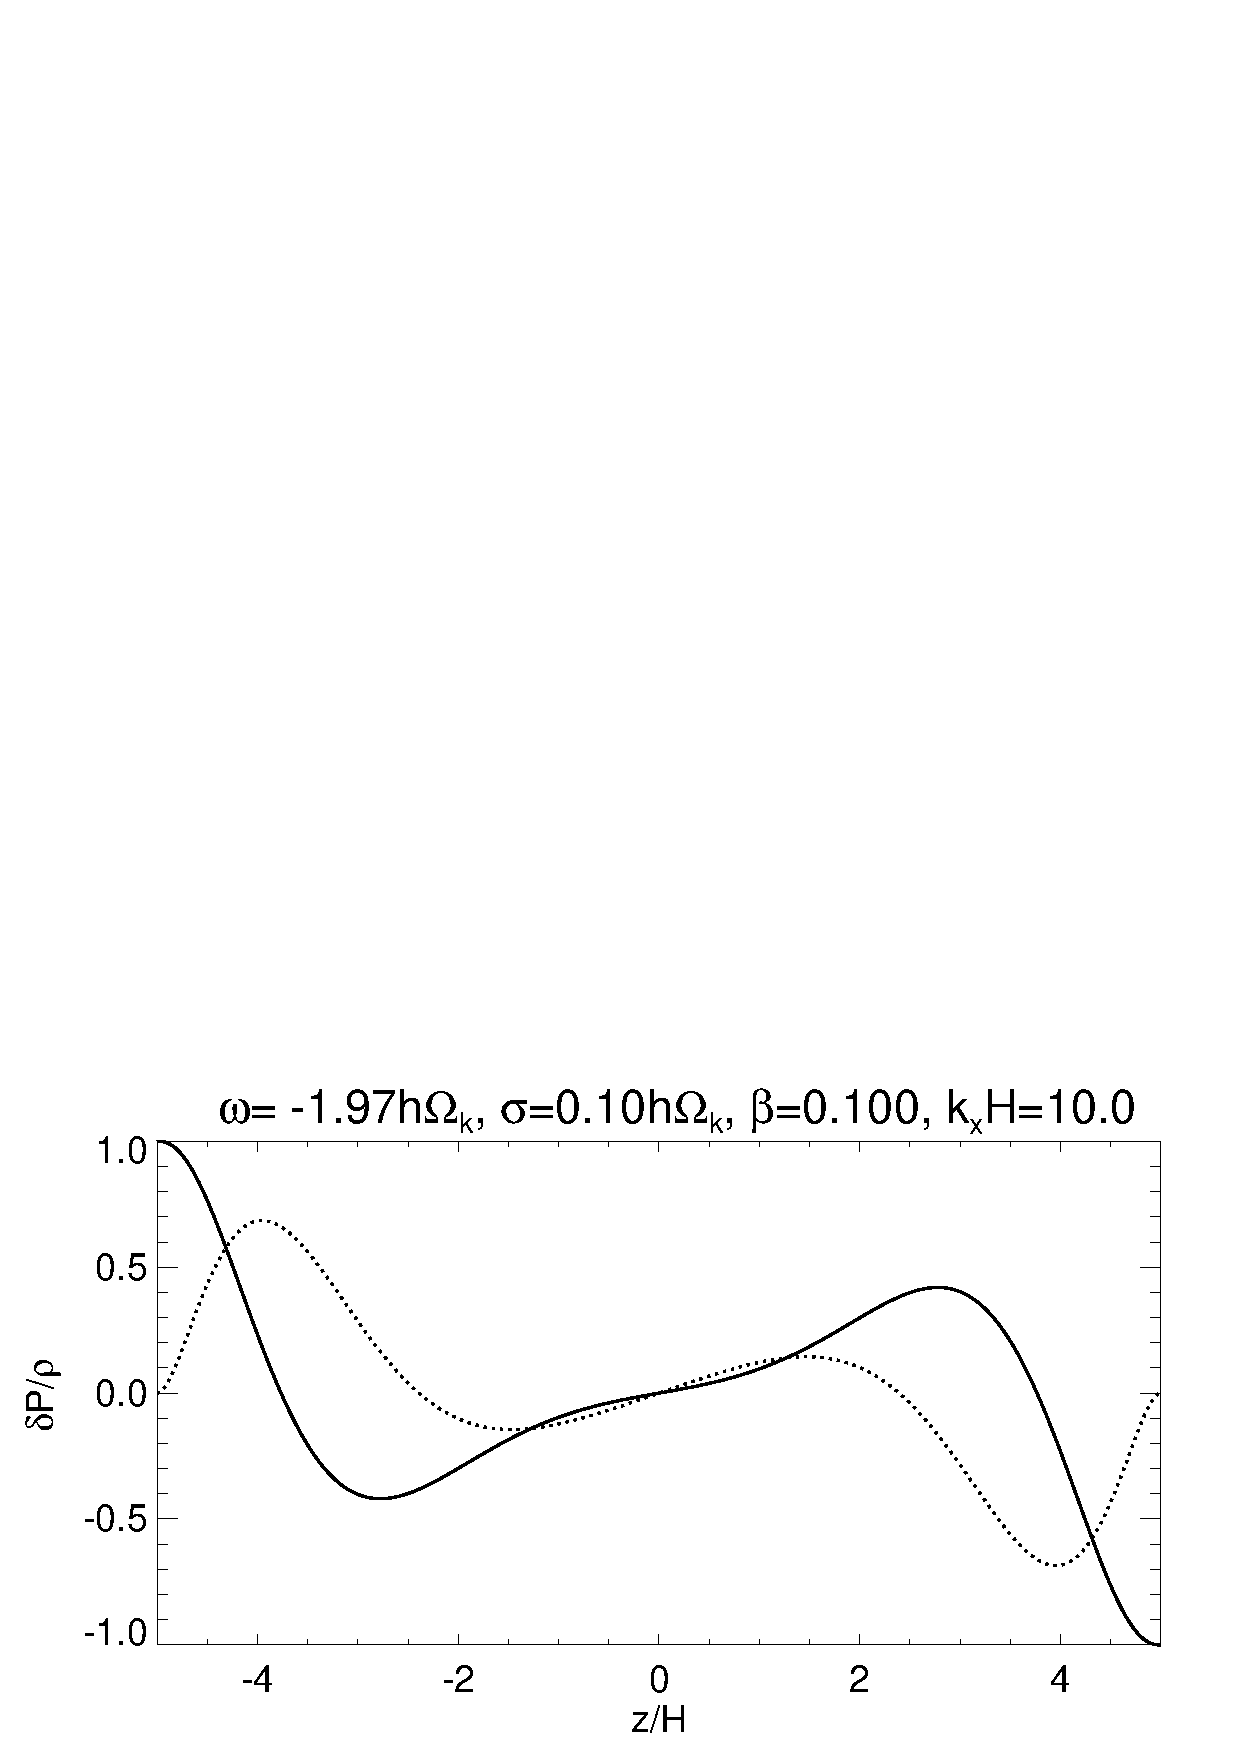
\includegraphics[width=\linewidth,clip=true,trim=0cm 1.75cm 0cm
  0cm]{figures/eigenvectorW_beta0d1} 
  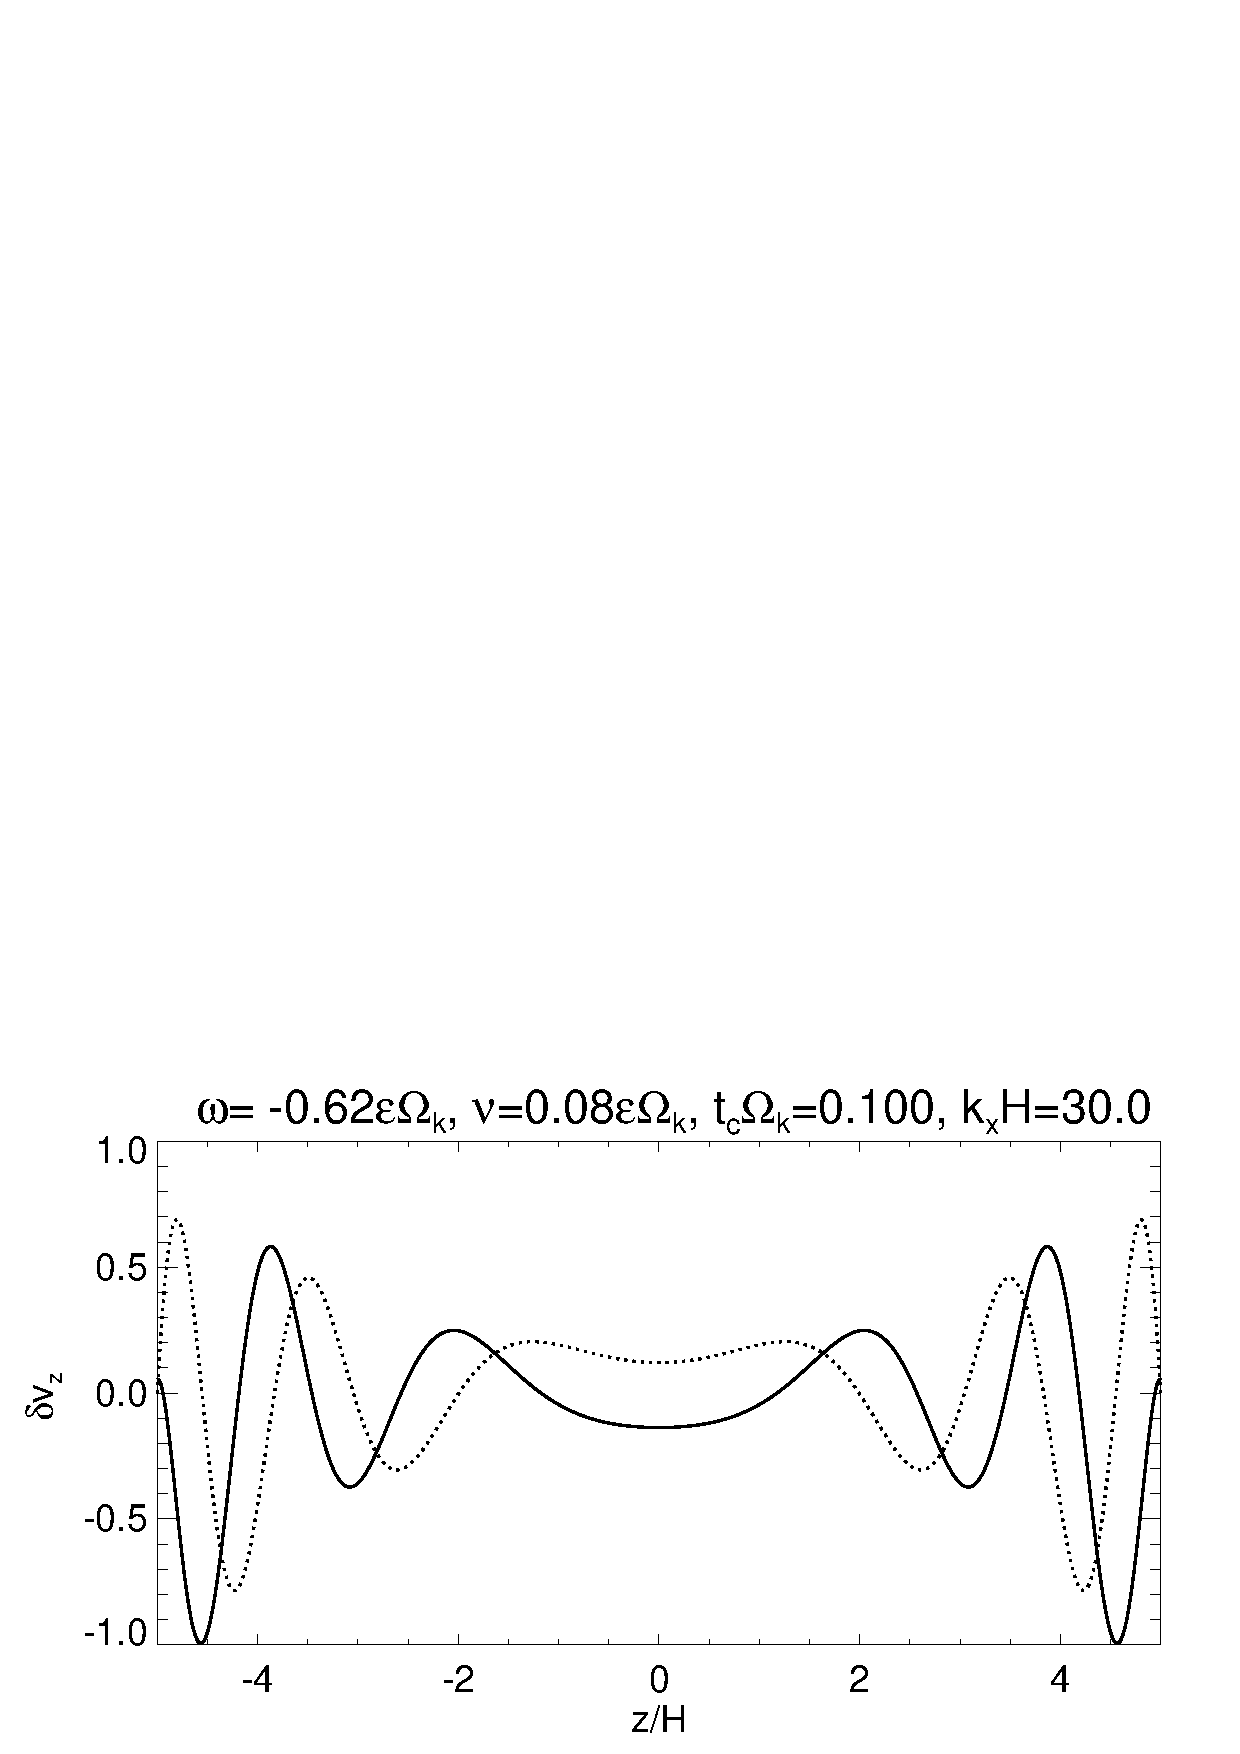
\includegraphics[width=\linewidth,clip=true,trim=0cm 0cm 0cm
  1cm]{figures/eigenvectorvz_beta0d1}
  \caption{Same as Fig. \ref{lowfreq_eigenfunc} but with a
    thermal relaxation timescale $\beta=0.1$. 
    \label{lowfreq_eigenfunc_cool}
  }
\end{figure}

\begin{figure}
  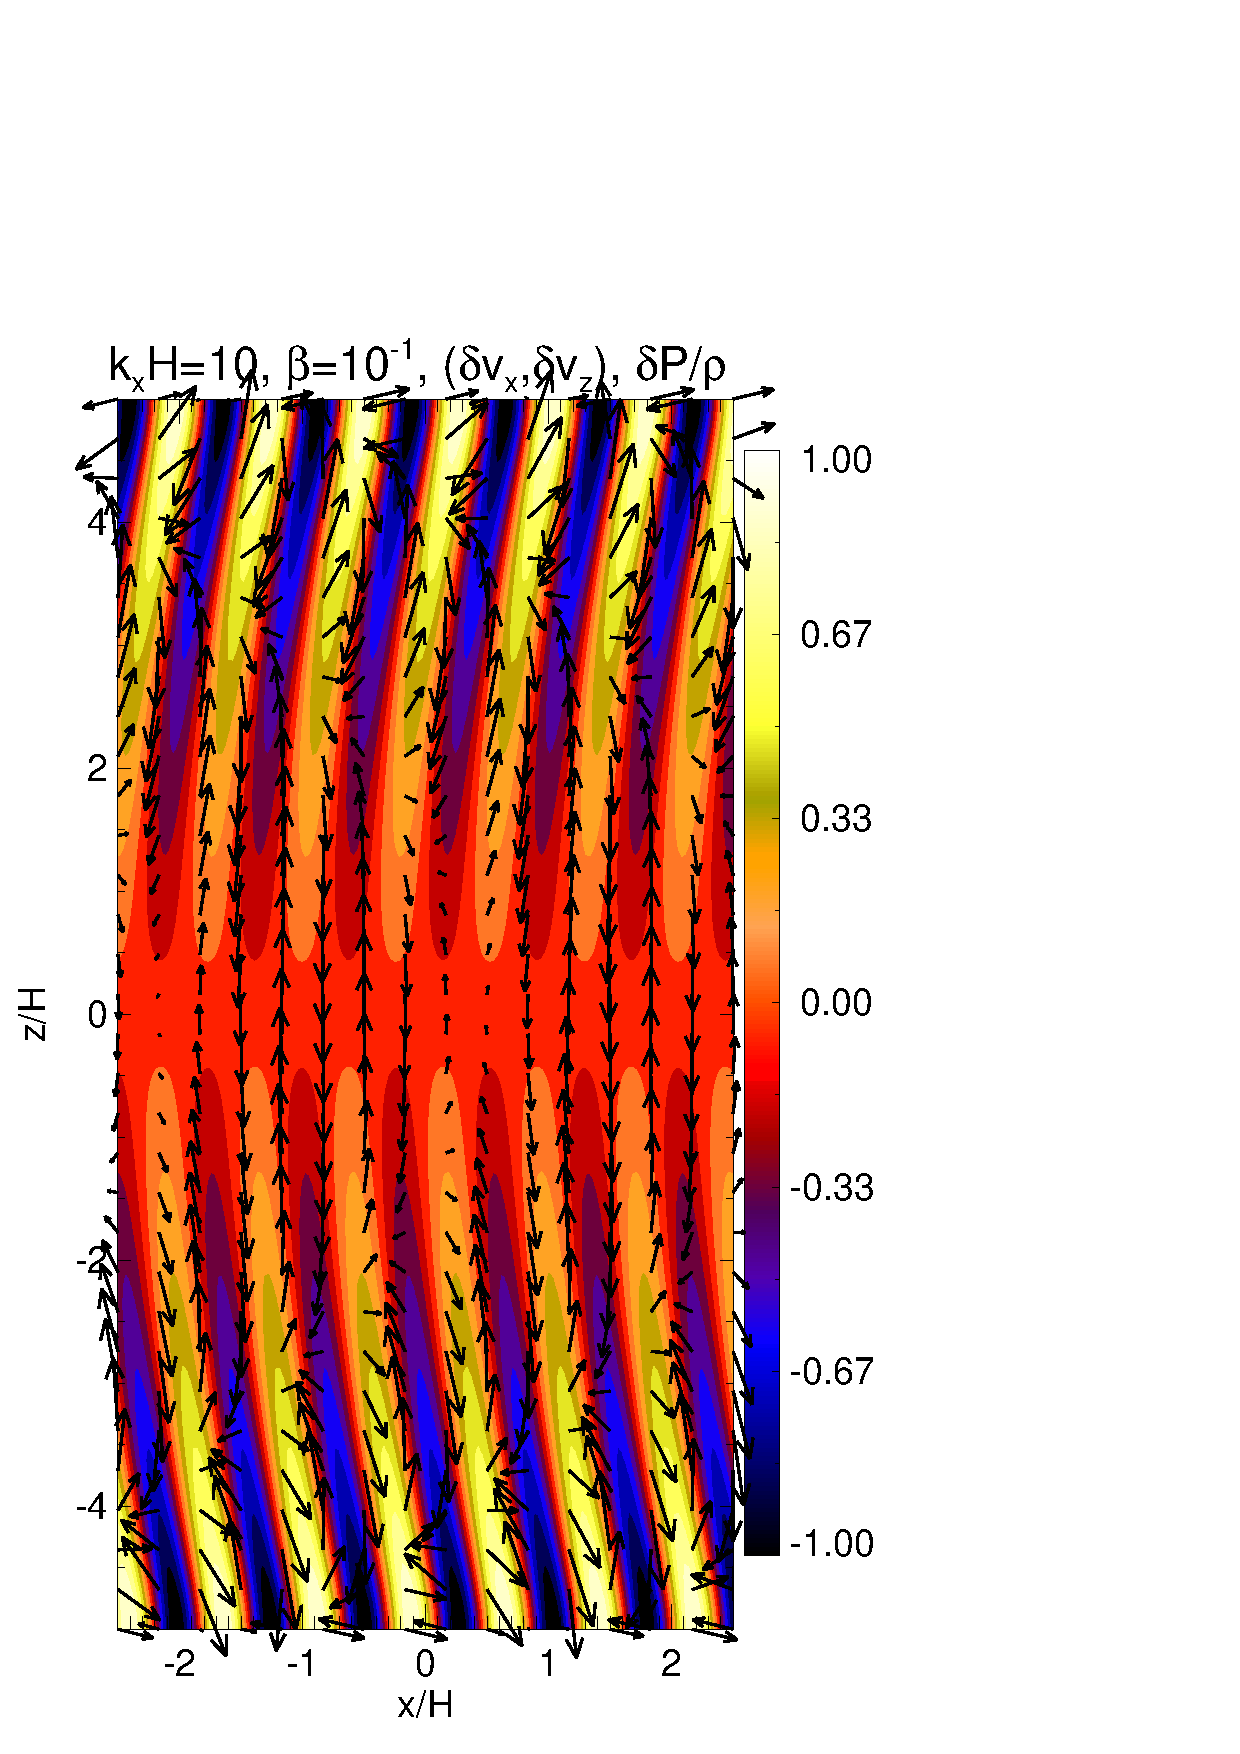
\includegraphics[scale=0.345,clip=true,trim=0cm 0cm 3.1cm
  0cm]{figures/result2d_vel_cool}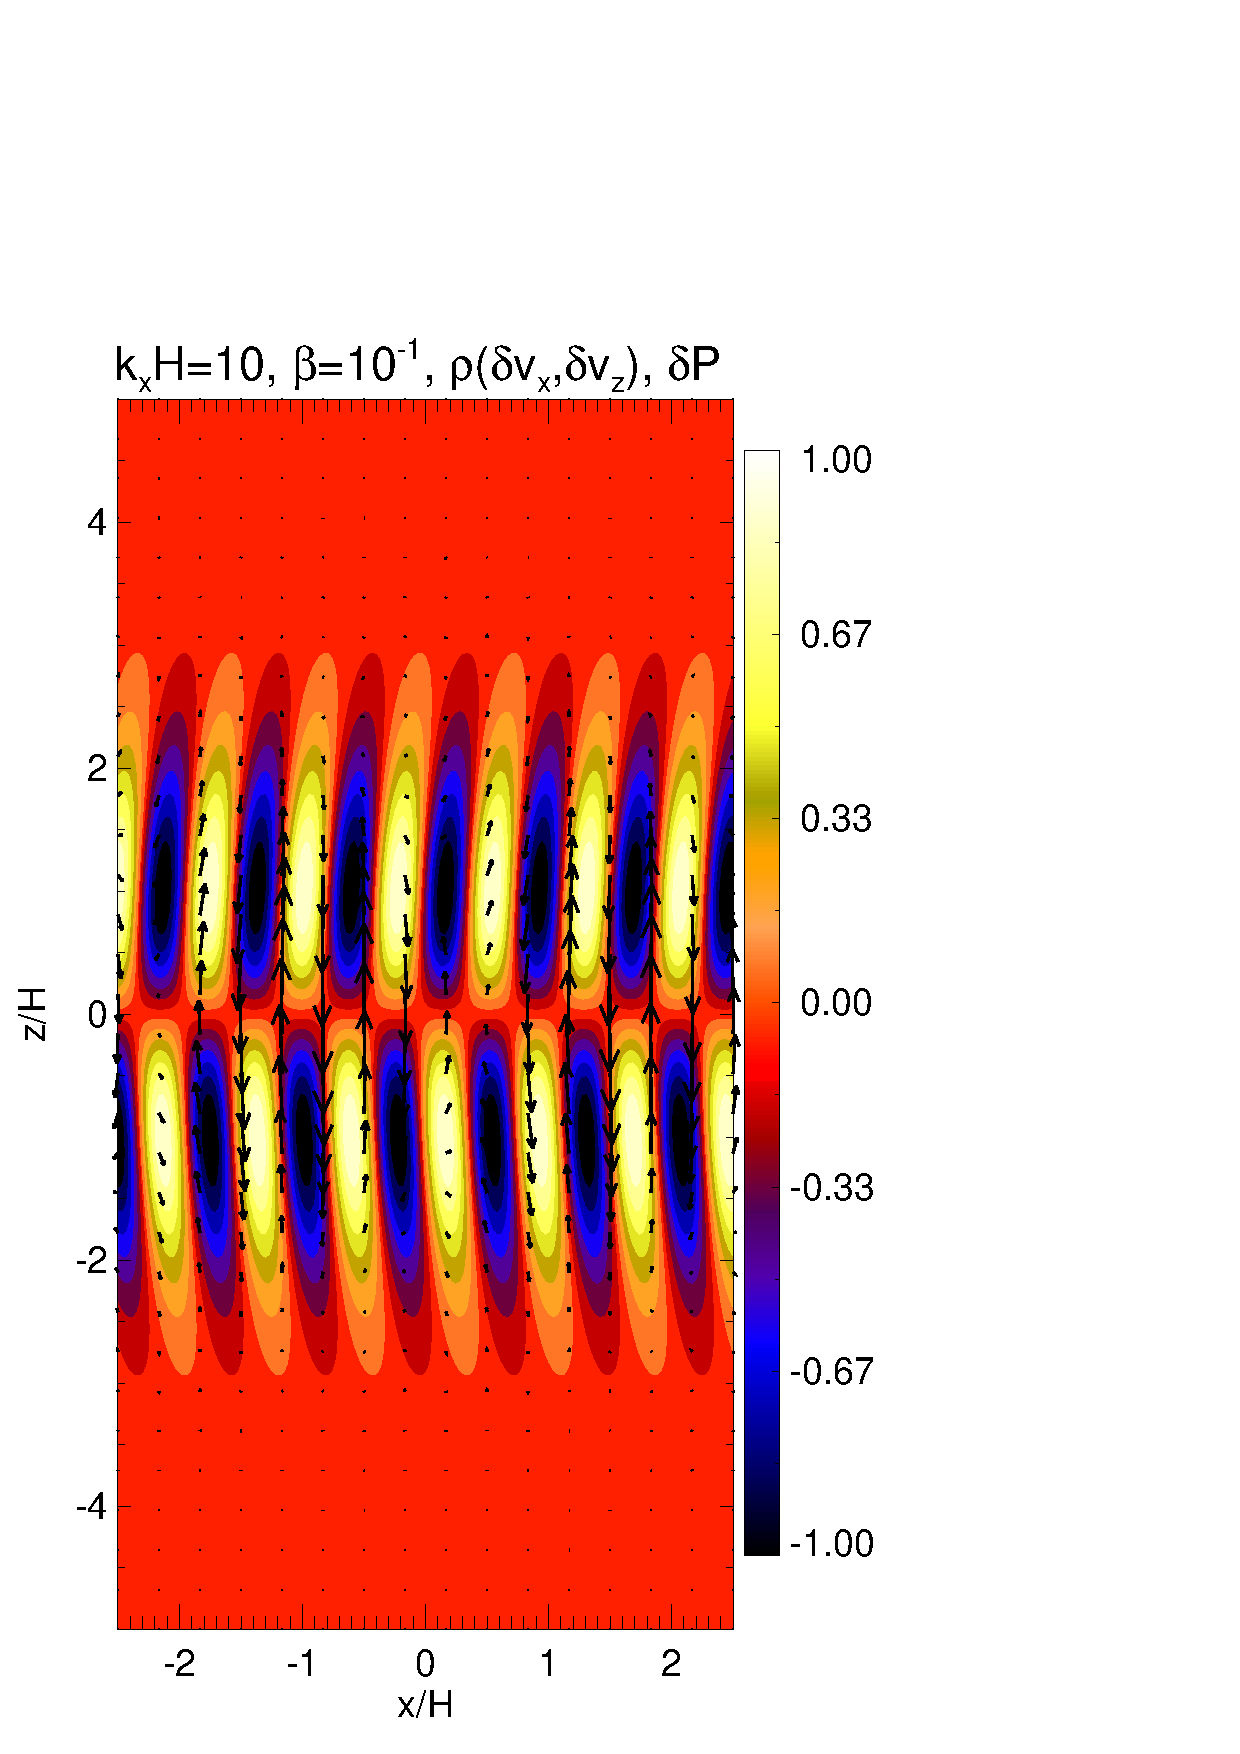
\includegraphics[scale=0.345,clip=true,trim=1.9cm 0cm 0cm
  0cm]{figures/result2d_mom_cool} 
  \caption{Same as  Fig. \ref{lowfreq_eigenfunc_2d} but with a thermal
    relaxation timescale $\beta=0.1$. 
    \label{lowfreq_eigenfunc_2d_cool}
  }
\end{figure}

\subsection{Critical thermal relaxation
  timescale}\label{bcrit_num_test}
We now test the critical thermal relaxation timescale given by
Eq. \ref{iso_vsi_cond}. We follow the fundamental mode by starting
from eigenvalues for $\beta=10^{-3}$ and slowly increase the thermal
relaxation timescale up to $\beta=10^3$. Fig. \ref{bcrit_compare1}
show the obtained growth rates, together with the critical 
thermal relaxation timescale $\beta_\mathrm{crit}=0.125$ for our
fiducial disk parameters.   

For $5\lesssim\khat\lesssim30$, we find $\beta_\mathrm{crit}$ provides
an accurate prediction of the upper limit to the thermal relaxation 
timescale for the fundamental mode. For smaller $\khat$, 
$\beta<\beta_\mathrm{crit}$ the VSI can operate slightly beyond
$\beta_\mathrm{crit}$ (recall that $\beta_\mathrm{crit}$ was derived
by assuming $\khat\gg 1$). For $\khat\geq 50$, we find perturbations
acquire large amplitudes near the vertical boundaries. Complications
% to our simple solution procedure 
may arise from surface modes. Nevertheless, growth rates rapidly
decrease as $\beta$ approach and increase beyond
$\beta_\mathrm{crit}$.  

Fig. \ref{bcrit_compare1} shows that $\beta_\mathrm{crit}$ provides a  
practical indication for the maximum thermal relaxation timescale to
permit the fundamental VSI. % From our discussion in 
% \S\ref{therm_relax_eff}, which indicate the fundamental mode typically
% dominant 
\cite{nelson13} found a thermal relaxation timescale of $\beta\gtrsim
0.6$ stabilized the VSI in non-linear hydrodynamic simulations. This 
is consistent with our results.   

It is interesting to note that there is a thermal relaxation timescale that
maximizes the mode decay rate for $1\lesssim \khat \lesssim 30$. Here,
it is $\beta\simeq1$---$2$ or about $0.1$---$0.3$ orbital
periods. This is in fact consistent with Fig. 12 of \cite{nelson13}
where the perturbed kinetic energy in their numerical simulations was
observed to decay most rapidly for a thermal timescale of $\sim 0.1$
orbits.     

%implications for nonlinear sims?

\begin{figure}
   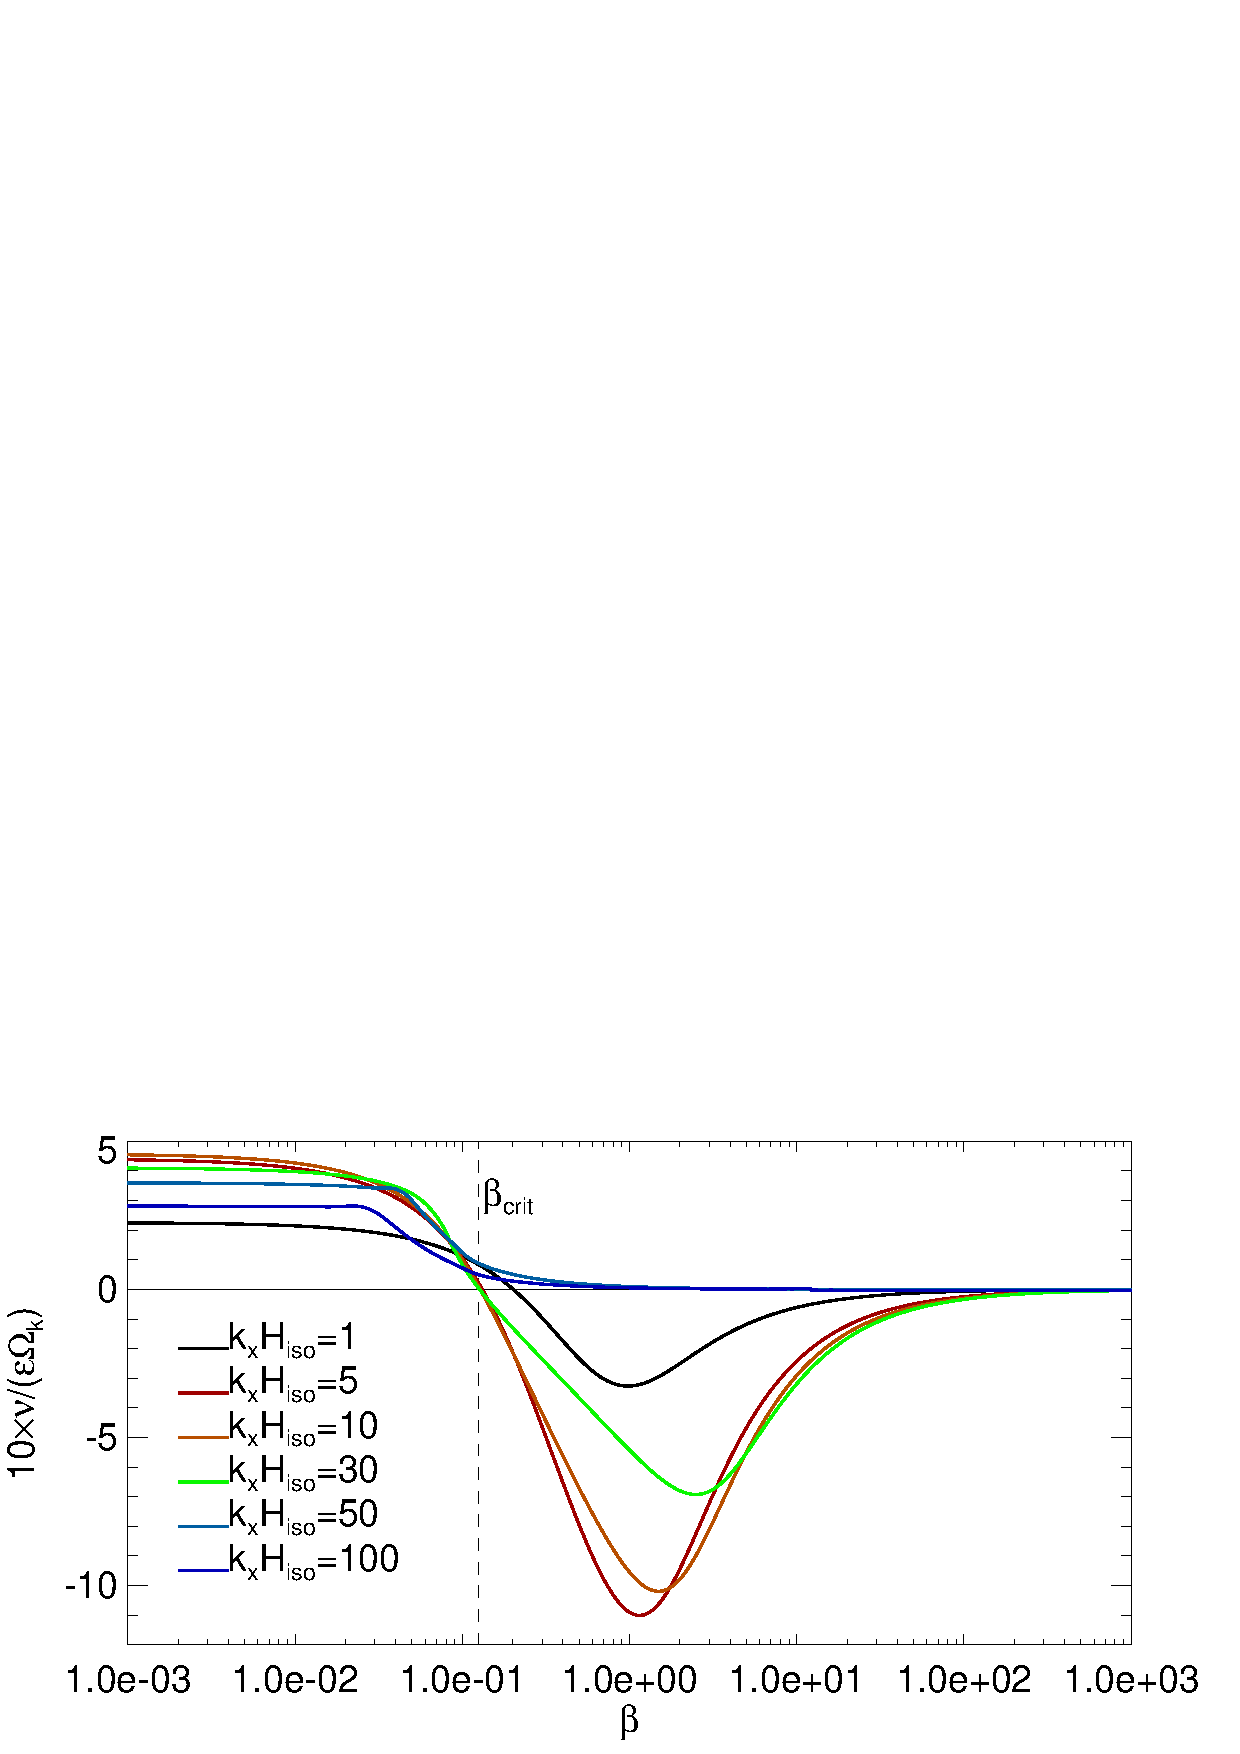
\includegraphics[width=\linewidth]{figures/gcorr_compare2} 
   \caption{Growth rate of the fundamental VSI in the fiducial disk
     model as a function of the thermal relaxation timescale $\beta$
     The vertical line
     is the critical thermal timescale $\beta_\mathrm{crit}$  obtained
     from Eq. \ref{iso_vsi_cond}. 
     \label{bcrit_compare1}}   
 \end{figure} 


% may need to explain why choose k=10
% bcrit independent of k for k>>1 
% for some parameter regimes (e.g. large q, large epsilon) 
% behavior at larger kx and finite bcool not understood. 
We further test the dependence of the critical thermal relaxation timescale 
$\beta_\mathrm{crit}$ on disk parameters
(Eq. \ref{iso_vsi_cond}).  We use the previous case study as a
reference point and vary $q\in[-0.2,-1.2]$, 
$\gamma\in[1.2,2.0]$, and $\epsilon\in[0.02,0.1]$
separately. Here, we use a wavenumber $\khat=10$, for which we
find growth rates reach zero for the range of disk parameters
considered, so that a numerical $\beta_\mathrm{crit}$ can be defined precisely. 

The numerically obtained $\beta_\mathrm{crit}$ is shown in
Fig. \ref{bcrit_compare} in comparison with Eq. \ref{iso_vsi_cond}.
Our numerical results generally agree with Eq. \ref{iso_vsi_cond}. The
agreement improves with decreasing  $|q|$,  $\epsilon$ and increasing
$\gamma$, i.e. weaker instability. There is a noticeable difference
as $\gamma\to1$ because the derivation of $\beta_\mathrm{crit}$
assumed $\gamma>1$.   

Fig. \ref{bcrit_compare}, together with the previous section
(Fig. \ref{bcrit_compare1}), shows that $\beta_\mathrm{crit}$ as given
by Eq. \ref{iso_vsi_cond} characterizes the thermal timescale below
which perturbations are effectively isothermal 
so that the VSI operates. 

% From the previous section (Fig. \ref{relax_eigenW_num}) we
% expect that for other wavenumbers,  still gives a characteristic
% thermal timescale below which the perturbations are effectively
% isothermal. 


\begin{figure}
  \includegraphics[width=\linewidth,clip=true,trim=0cm 0.cm 0cm
  0cm]{figures/bcrit_compare_q.ps} 
  \includegraphics[width=\linewidth,clip=true,trim=0cm 0.0cm 0cm
  0.8cm]{figures/bcrit_compare_g.ps}
  \includegraphics[width=\linewidth,clip=true,trim=0cm 0.0cm 0cm
  0.8cm]{figures/bcrit_compare_e.ps} 
  \caption{Dependence of the upper limit to the thermal relaxation timescale
    $\beta_\mathrm{crit}$ for the fundamental VSI mode on disk
    parameters. The fiducial parameters are $\Gamma=1.011$,
    $\gamma=1.4$ and $(p,q,\epsilon)=(-1.5,-1,0.05)$. Top: varying
    $q\in[-1.2,-0.2]$; middle: varying $\gamma\in[1.2,2.0]$; bottom:
    varying $\epsilon\in[0.02,0.1]$. The perturbation wavenumber is
    $\khat=10$.  
    \label{bcrit_compare}}  
\end{figure}

\subsection{Vertically non-isothermal disks} 
We briefly consider vertically non-isothermal disks with 
$\Gamma=1.4$ and $(p,q,\epsilon)=(0,-1,0.05)$ as simulated in
\cite{nelson13}. In this case we set $\zmax=0.99H_s$.  

Fig. \ref{gcorr_compare_vnoniso} plots the fundamental VSI growth
rates as a function of $\beta$ for $\gamma\in[1.4,2.5]$. In agreement
with \citeauthor{nelson13}, in  
the neutrally-stratified case $\gamma=\Gamma$ the disk is unstable 
even for $\beta\gg 1$. (Note that in the adiabatic limit 
this disk can be unstable according to the
Solberg-Hoiland criterion, Eq. \ref{solberg2}.) 

For $\gamma>\Gamma$, i.e. stably stratified disks,
Fig. \ref{gcorr_compare_vnoniso} shows that introducing finite thermal
relaxation rapidly stabilizes the fundamental mode. This is
similar to that observed for nearly vertically isothermal disks
(Fig. \ref{bcrit_compare1}). For $\gamma=1.7,\,2.0,\,2.5$, growth
rates reach zero at  $\beta\simeq0.17,\,0.083,\,0.045$, respectively.
Interestingly, these values are equal to
$\epsilon|q|/(\gamma-\Gamma)$. This suggests that the critical thermal
relaxation timescale for vertically non-isothermal disks can also be
estimated by Eq. \ref{iso_vsi_cond} but with $\gamma-1$ replaced by
$\gamma-\Gamma$. 

\begin{figure}
  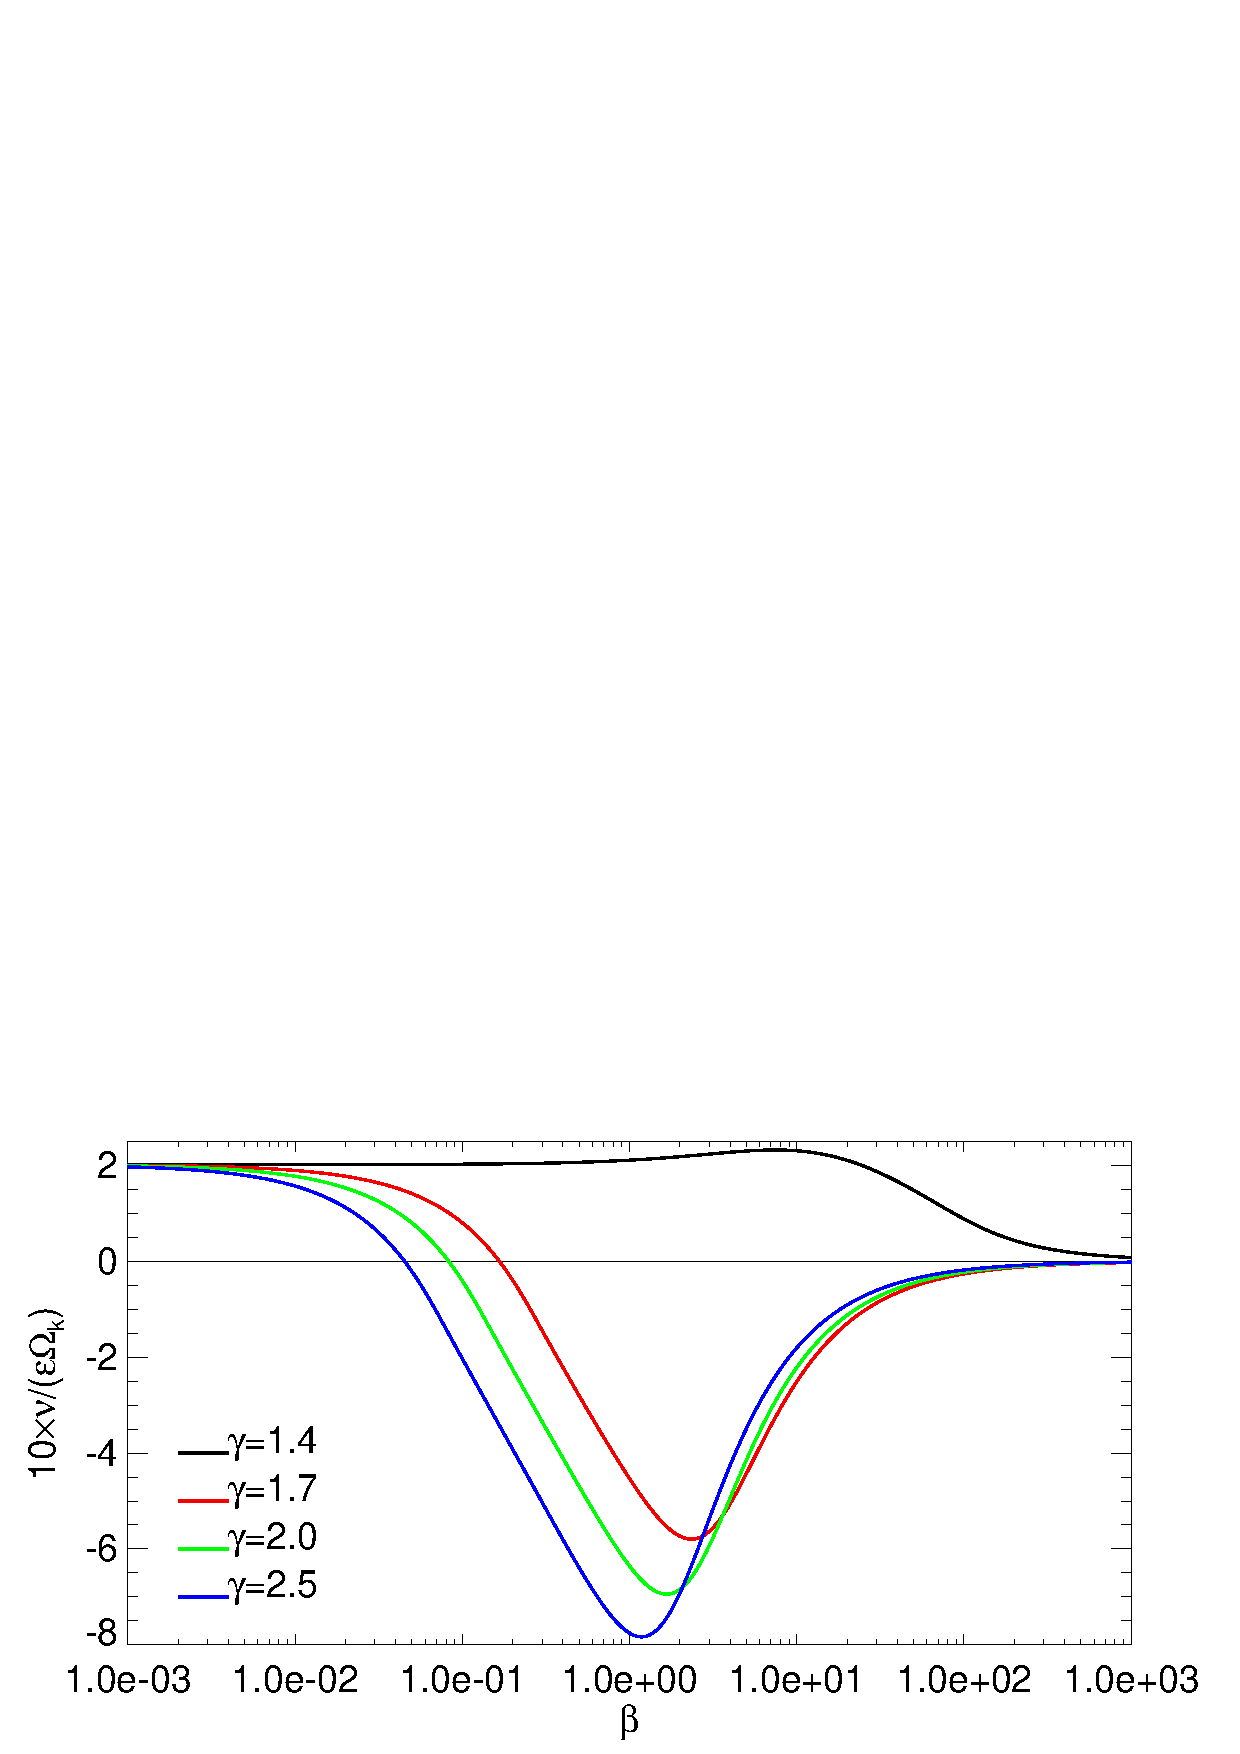
\includegraphics[width=\linewidth,clip=true,trim=0cm 0cm 0cm
  0cm]{figures/gcorr_compare_vnoniso2}
  \caption{Growth rate of the fundamental VSI mode as a function of
    the thermal relaxation timescale $\beta$, in vertically
    non-isothermal disks with $\Gamma=1.4$ and
    $\gamma\in[1.4,2.5]$. The disk is neutrally
    stratified for $\gamma=1.4$ and stably stratified for
    $\gamma>1.4$. Other disk parameters are
    $(p,q,\epsilon)=(0,-1,0.05)$ and the perturbation wavenumber is
    $\khat=30$.  
    \label{gcorr_compare_vnoniso}}
\end{figure}












